\documentclass{cubeamer}
\setbeamercovered{transparent} % preview text when using \uncover
\usepackage{etoolbox} % for precise adjustments within environments 
\usepackage[sfdefault,semibold]{FiraSans}

\usepackage[normalem]{ulem} % fancy underlines and stuff 
\usepackage[dvipsnames, table]{xcolor} % named colors 

% command to strike out text in red
\renewcommand{\ULthickness}{1.5pt}  % making striketrhough bolder
\newcommand<>\redout[1]{\alt#2{\bgroup\markoverwith
{\textcolor{red}{\rule[0.5ex]{2pt}{0.8pt}}}\ULon{#1}}{{#1}}}

\linespread{0.85} % tighter line spacing 

\newcommand<>{\hlonly}[1]{\alt#2{\hl{#1}}{#1}}

% Decreasing itemize environment font size
\setbeamerfont{itemize/enumerate body}{size=\small}
\setbeamerfont{itemize/enumerate subbody}{size=\footnotesize}

% increasing bullet size 
\setbeamertemplate{itemize item}{\small$\bullet$}
\setbeamertemplate{itemize subitem}{\footnotesize$\circ$}
\setbeamertemplate{itemize subsubitem}{\tiny$-$}

\setbeamerfont{frametitle}{size=\LARGE}

% This should work for item spacing
\let\olditemize\itemize
\renewcommand{\itemize}{%
  \olditemize
  \setlength{\itemsep}{0pt plus 0pt minus 0pt}%
  \setlength{\parskip}{0pt}%
  \setlength{\parsep}{0pt}%
  \setlength{\topsep}{0pt}%
  \setlength{\partopsep}{0pt}%
}

% Also patch enumerate for consistency
\let\oldenumerate\enumerate
\renewcommand{\enumerate}{%
  \oldenumerate
  \setlength{\itemsep}{0pt plus 0pt minus 0pt}%
  \setlength{\parskip}{0pt}%
  \setlength{\parsep}{0pt}%
  \setlength{\topsep}{0pt}%
  \setlength{\partopsep}{0pt}%
}

% Make item spacing match normal text
\setbeamertemplate{itemize/enumerate body begin}{%
    \vspace{-0.5\baselineskip}%
}
% \setbeamertemplate{itemize/enumerate subbody begin}{%
%     \vspace{-0.5\baselineskip}%
%     %
% }

\newcommand<>{\uncovergraphics}[2][{}]{
    % Taken from: <https://tex.stackexchange.com/a/354033/95423>
    \begin{tikzpicture}
    \node[anchor=south west,inner sep=0] (B) at (4,0)
        {\includegraphics[#1]{#2}};
    \alt#3{}{%
        \fill [draw=none, fill=white, fill opacity=0.9] (B.north west) -- (B.north east) -- (B.south east) -- (B.south west) -- (B.north west) -- cycle;
    }
    \end{tikzpicture}
}

\setcounter{tocdepth}{2} % Only sections and higher will appear
\setbeamerfont{subsection title}{shape=\itshape, series=\mdseries}

\usepackage{graphicx}

\usepackage[style=ieee,backend=biber]{biblatex} % better citations 
\setbeamerfont{bibliography item}{size=\tiny}
\setbeamerfont{bibliography entry author}{size=\tiny}
\setbeamerfont{bibliography entry title}{size=\tiny}
\setbeamerfont{bibliography entry location}{size=\tiny}
\setbeamerfont{bibliography entry note}{size=\tiny}

\renewcommand*{\bibfont}{\tiny\linespread{0.85}} % changed

% \setlength{\bibitemsep}{0pt plus 0pt minus 0pt} % Changed? 
\setbeamertemplate{frametitle continuation}{}

% \usepackage[draft]{animate}
\usepackage{animate}

% \usepackage{multirow}
\newcolumntype{R}[1]{>{\raggedleft\arraybackslash}p{#1}}

\newcommand{\e}[0]{\mathrm{e}}                      % math e 
% \usepackage{wrapfig} % environment to wrap text around a figure
\usepackage{emoji}
\usepackage{soul} % highlighting and such
% \includeonlyframes{gnss_viability}
\addbibresource{biblio.bib}
\title{\textbf{First Results Using Time-of-Flight Positioning for Specular Meteor Radar: Analysis of an Experimental Campaign}}
\subtitle[AGU26, SA22B]{Upper Atmosphere Research Advanced by Emerging Technologies I Oral\\AGU26, SA22B}
\author[J. Monaco]{J. Monaco\(^1\) \\ Scott E. Palo\(^1\) \\ Kenneth Obenberger\(^2\)}
\date{December 8th, 2026} 
\institute[University of Colorado Boulder]{\scriptsize \(^1\)University of Colorado Boulder, \\ Ann and H.J. Smead Department of\\ Aerospace Engineering Sciences \\ ~ \\ 
\(^2\)Air Force Research Lab, \\ Space Vehicles Directorate}
\titlegraphic{
    \begin{tikzpicture}[remember picture,overlay]
        \node[anchor=east] at ([yshift=-1cm]current page.east) {
            \scalebox{1}[1]{\adjincludegraphics[width=0.65\textwidth]{img/title_graphic.pdf}}
        };
    \end{tikzpicture}
}

\hypersetup{
	pdftitle={An Alternative to Interferometry: Developing a Time-of-Flight Position Solution for Specular Meteor Radar Networks},
	pdfauthor={J. Monaco}}
\begin{document}

\maketitle

\begin{frame}[label=gnss_conclusions]
    \frametitle{Summary: Time-of-Flight (TOF) Positioning}
    % \begin{columns}
    %     \begin{column}{1.1\textwidth}
    %         \alert{Specular meteor radar} systems use interferometry to locate reflective meteors and probe the MLT \\ ~ \\
    %     \end{column}
    % \end{columns}
    \begin{columns}
        \begin{column}{0.7\textwidth}
            \alert{Specular meteor radar} systems use interferometry to locate reflective meteors and probe the MLT \\ ~ \\

            \uncover<2->{\alert{Interferometry is challenging} to calibrate, derive uncertainties} \\ ~ \\
            % \begin{itemize}
            %     \item[$\blacktriangleright$] Makes deployment, operation, and analysis difficult 
            % \end{itemize}}

            \uncover<3->{\alert{TOF positioning} can provide precise position estimates %
            \begin{itemize}  %\vspace{-\baselineskip}%
                \item Only uses range measurements
                \item {No calibration} \(\xrightarrow[]{}\) {easier deployments}
                \item {Easily derived uncertainties} \(\xrightarrow[]{}\) {better analysis}
                \item Robust to noise \(\xrightarrow[]{}\) {fewer observations discarded}
            \end{itemize}}

            \uncover<4->{\alert{Few system changes required}: larger \textcolor{red}{\textbf{RX}} arrays} \\ ~ \\ 

            \uncover<5->{Could \alert{replace or supplement} interferometry} \\ ~ \\

            \uncover<6->{An experimental campaign was attempted to directly compare positioning methods}

        \end{column}
        \begin{column}{0.4\textwidth}
            \centering
             \begin{tikzpicture}[anchor=(current bounding box.north)]
                \node[anchor=north, inner sep=0] (img) at (0,0) {
                    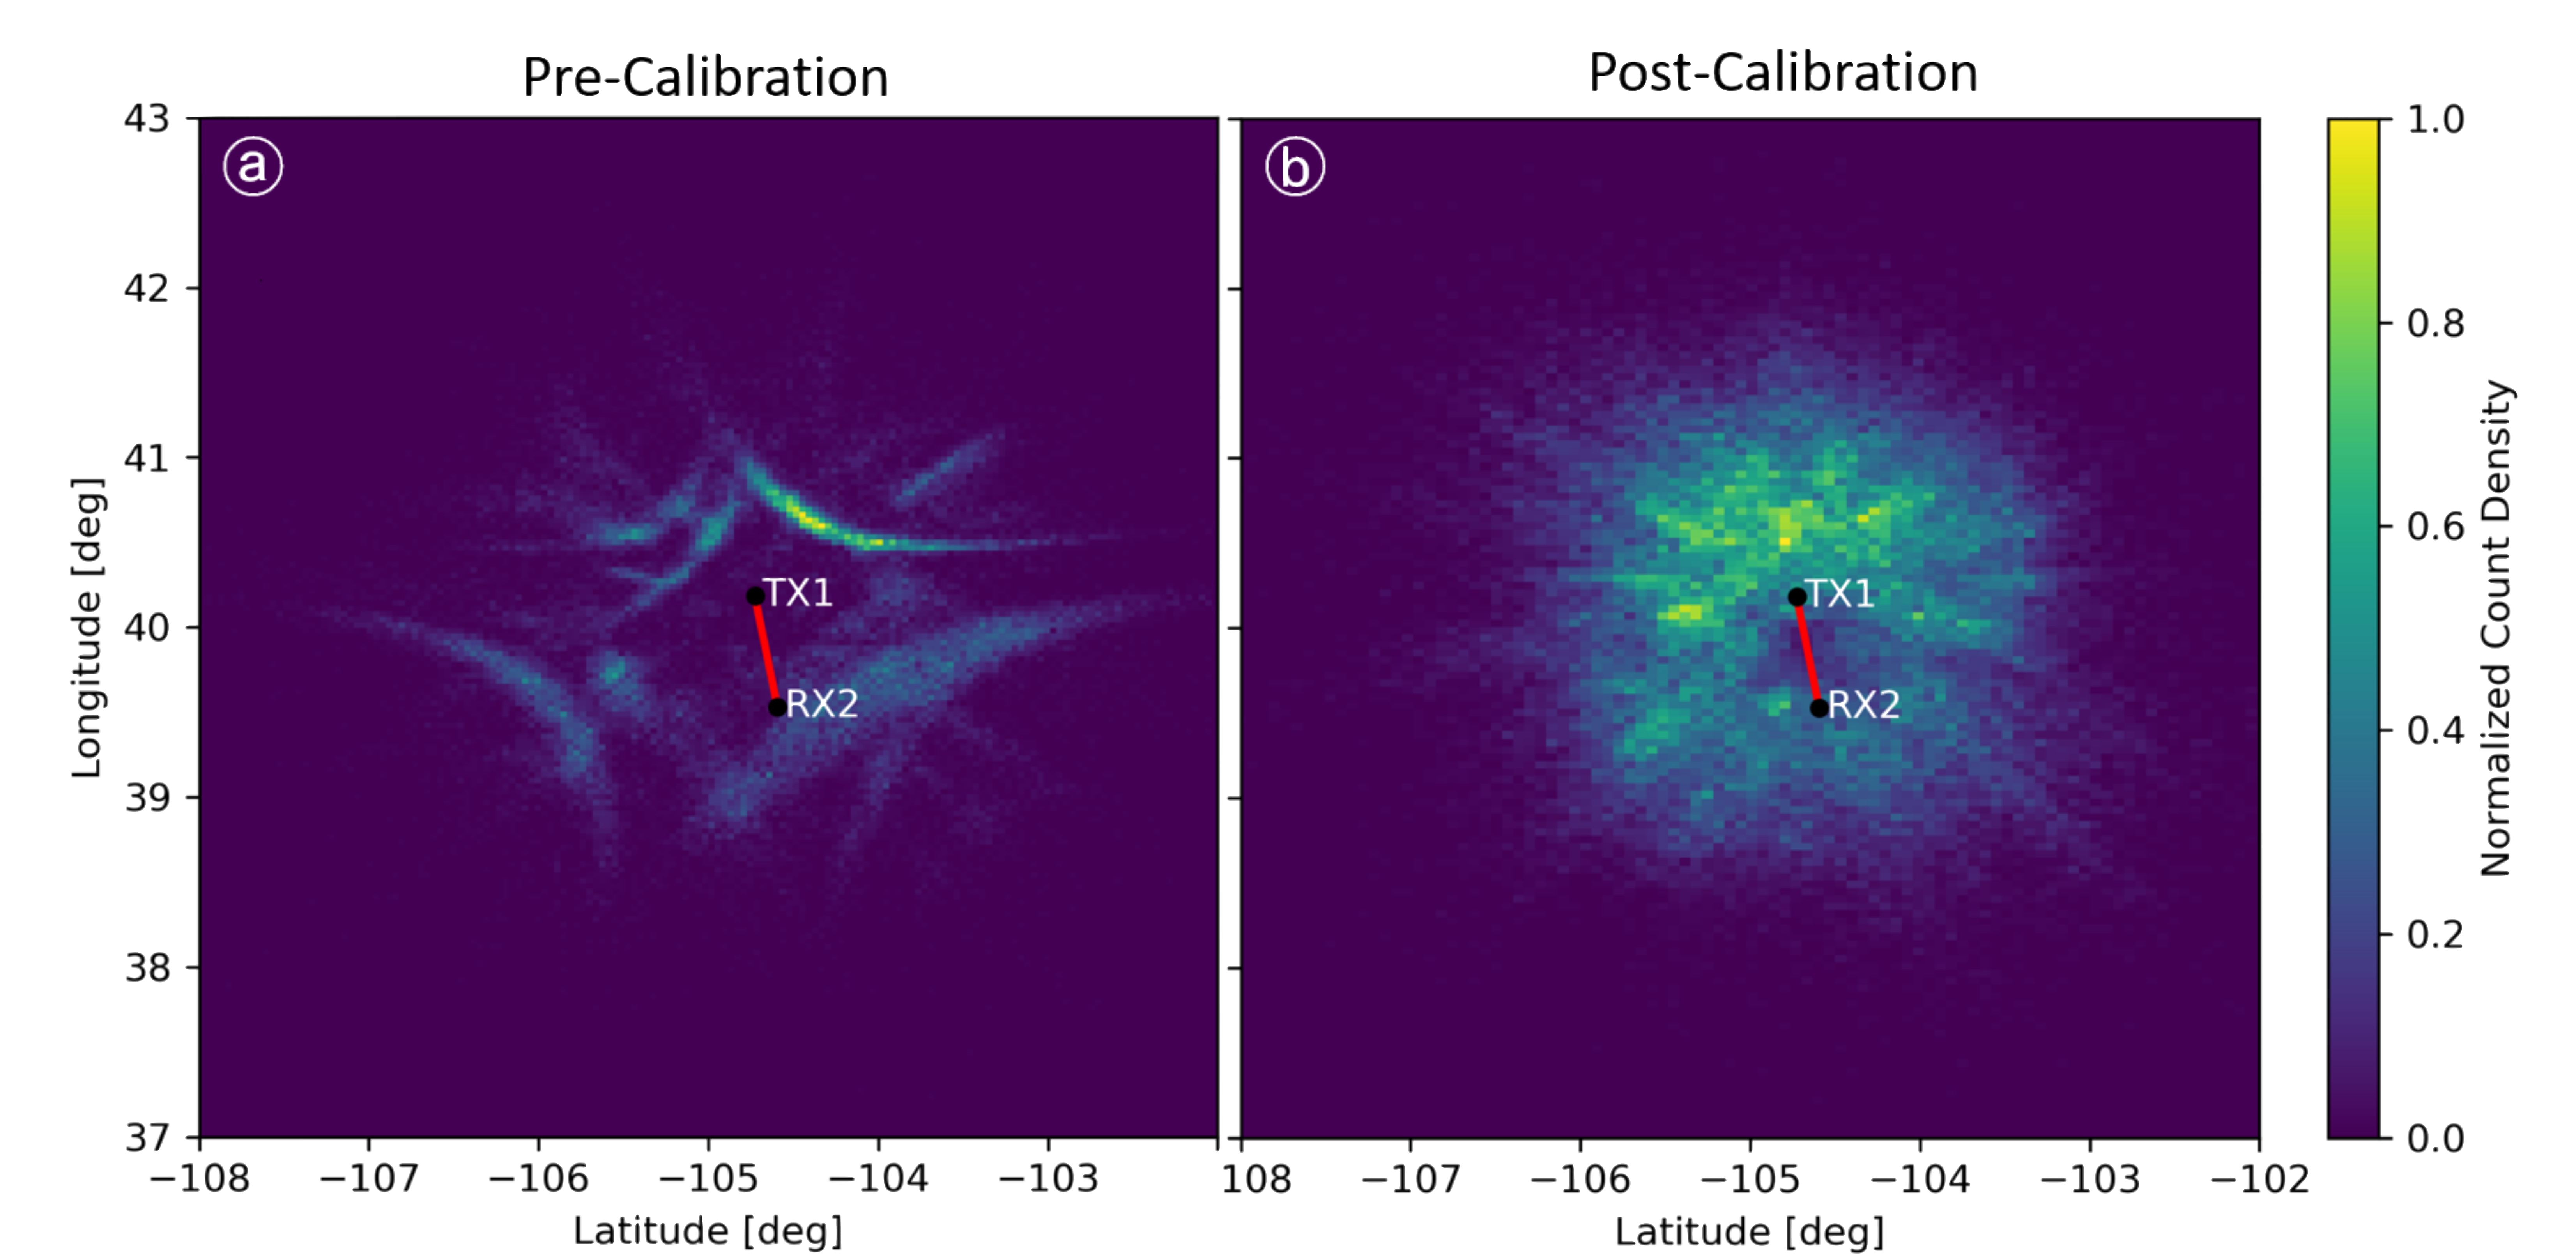
\includegraphics[width=0.85\linewidth]{img/calibration2.png}
                };
                \node[anchor=south, inner sep=2pt] at ([yshift=0.25cm, xshift=0.6cm]img.south) { 
                    {{{\fontsize{3}{3.4}\selectfont\raggedleft \textcolor{white}{\textit{Credit:} \citeauthor{marino_MeteorRadarPhase_2024}, \citeyear{marino_MeteorRadarPhase_2024} \cite{marino_MeteorRadarPhase_2024}}}}}
                };
            \end{tikzpicture}
            % 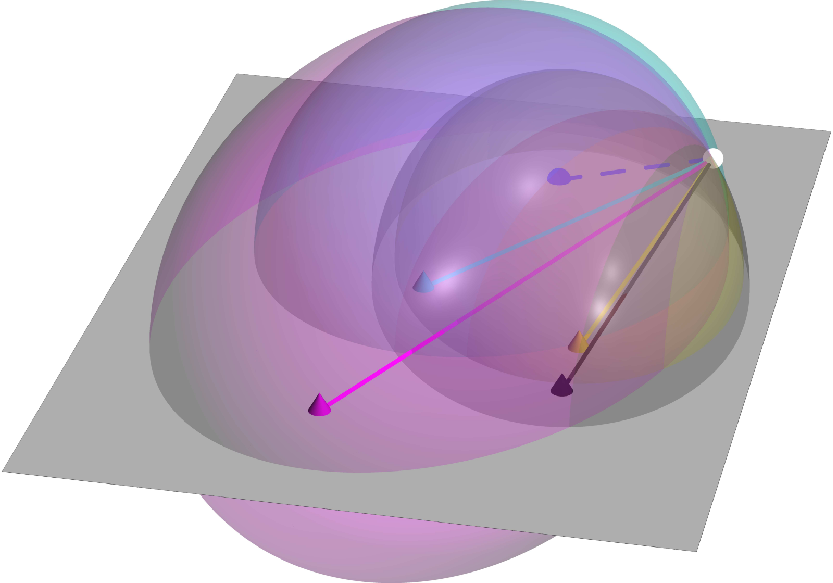
\includegraphics[width=0.65\linewidth]{img/4ellipsoids_compressed.pdf}
            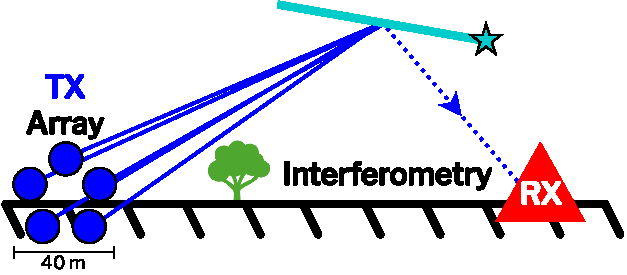
\includegraphics[width=\linewidth]{img/IF_basis_labeled.pdf}
            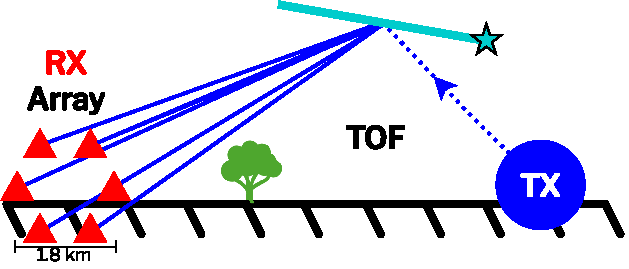
\includegraphics[width=\linewidth]{img/TOF_basis_labeled.pdf}
        \end{column}
    \end{columns}
\end{frame}

\section[Meteor Radar Background]{Meteor Radar Background}


\begin{frame}[label=basis]
    \frametitle{Basis of Meteor Radar}
    \begin{columns}
        \begin{column}{0.75\textwidth}
            \\ ~ \\ Using ground-based \textbf{\textcolor{blue}{transmitter}}s (\textcolor{blue}{\textbf{TX}}) and \textbf{\textcolor{red}{receiver}}s (\textcolor{red}{\textbf{RX}}):
            \begin{itemize}
                \item Ablating \textbf{\textcolor{cyan}{meteor trails}} act as reflective atmospheric tracers 
                \item \textcolor{red}{\textbf{RX}} compares the signal sent to the echo received
                \item Meteor and environmental parameters estimated 
            \end{itemize}
            % \hl{\textbf{No other way to \textit{densely} sample this region}} 
            \centering
            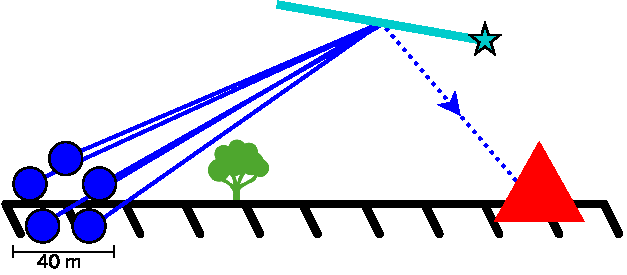
\includegraphics[width=0.85\textwidth]{img/IF_basis.pdf}
            % \begin{tikzpicture}
            %     \node[anchor=south west, inner sep=0] (image) at (0,0) {%
            %     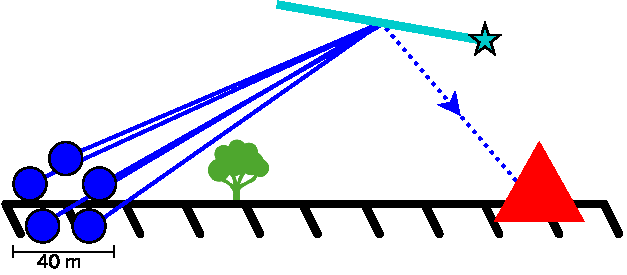
\includegraphics[width=0.85\textwidth]{img/IF_basis.pdf}};
            %     % \node<1->[circle, draw=yellow, fill=yellow!30, thick, minimum size=4mm] at ([xshift=1.05cm, yshift=0.5cm]image.west) {1};
            %     % \uncover<2->{\node[circle, draw=yellow, fill=yellow!30, thick, minimum size=4mm] 
            %     % at ([xshift=0.95cm, yshift=-1.1cm]image.north) {2};}
            %     % \uncover<3->{\node[circle, draw=yellow, fill=yellow!30, thick, minimum size=4mm] 
            %     % at ([xshift=-1.3cm, yshift=0.5cm]image.east) {3};}
            % \end{tikzpicture}
        \end{column}
        % \vrule{}
        \begin{column}{0.3\textwidth}
            \vspace{-10pt}
            \begin{center}%
                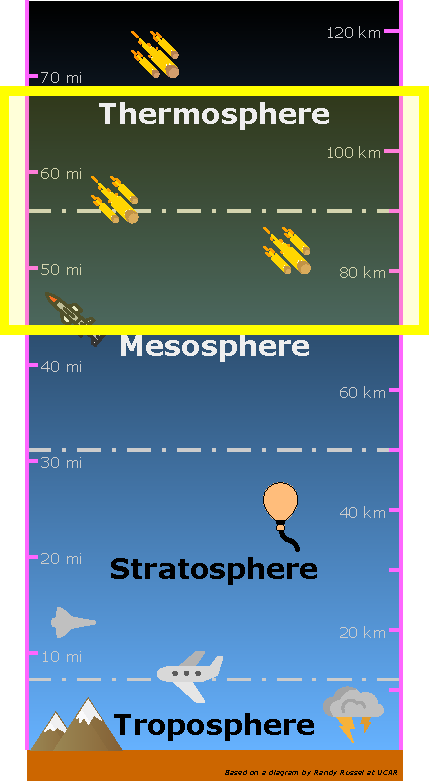
\includegraphics[height=0.65\textheight]{img/atmos_layers.pdf}
            \end{center}
            \footnotesize \vspace{-10pt}
            % \uncover<+->{Ultimate goal: \alert{Science!}
            % \begin{itemize} \scriptsize
            %     \item Seasonal trends
            %     \item Energy transport 
            %     \item Inform atmospheric models 
            % \end{itemize}}
        \end{column}
    \end{columns}
\end{frame}

\begin{frame}
    \frametitle{Final Products}
    \hspace*{-1cm}
    \fbox{\begin{minipage}[t]{0.4\paperwidth}
        \centering
        \textbf{Meteor Observations}
        \begin{columns}
            \begin{column}{0.35\linewidth}
                {\setbeamercovered{transparent=60}\noindent
                \begin{itemize}
                    \footnotesize
                    \item<0> Position
                    \item<0> Time
                    \item<0> Speed
                \end{itemize}}
            \end{column}
            \begin{column}{0.6\linewidth}
                {\setbeamercovered{transparent=60}\setlength{\leftmargini}{0pt}
                \begin{itemize}
                    \footnotesize
                    \item<0> Radial wind
                    \item<0> Diffusion coefficient
                    \item<0> Mass
                    \item<0> Trail orientation
                \end{itemize}}
            \end{column}
        \end{columns}
        \(\times1,000 +\) observations per hour... 
        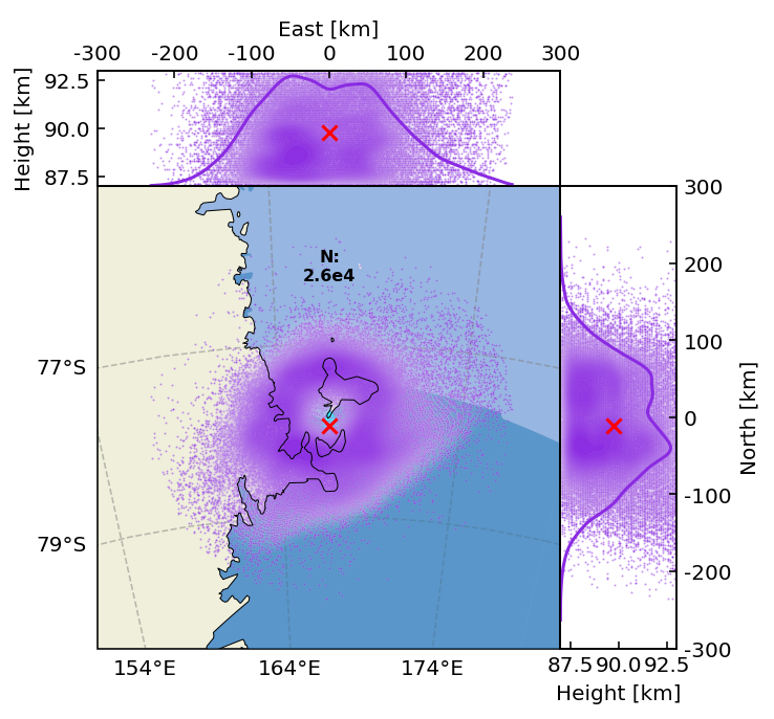
\includegraphics[width=0.8\linewidth]{img/mcmurdo_ortho.png} 
    \end{minipage}}%
    \begin{minipage}[t]{0.6\paperwidth}
        {\(\xrightarrow[Analyze]{Combine}\)}\uncover<2->{\textbf{\ \ Science}}
    \end{minipage}
    \begin{tikzpicture}[remember picture, overlay]
        \node<2->[anchor=south east] (image) at ([xshift=-0.5cm, yshift=0.5cm + 3cm + 5pt]current page.south east) {
            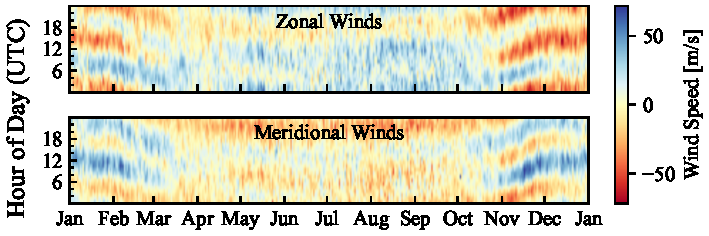
\includegraphics[width=5.5cm]{img/seasonal_trends.pdf}
        };
        \node<2-> at (image.center) {%
            \begin{tcolorbox}[width = 3cm, center, boxrule=0pt,colback=yellow,arc=0pt,auto outer arc,left=0pt,right=0pt,boxsep=0pt]
                \centering
                \footnotesize
                Wind time series
            \end{tcolorbox}
        };
        \node<2->[anchor=south east] (image) at ([xshift=-6.25cm - 5pt, yshift=0.5cm + 3.25cm + 5pt]current page.south east) {
            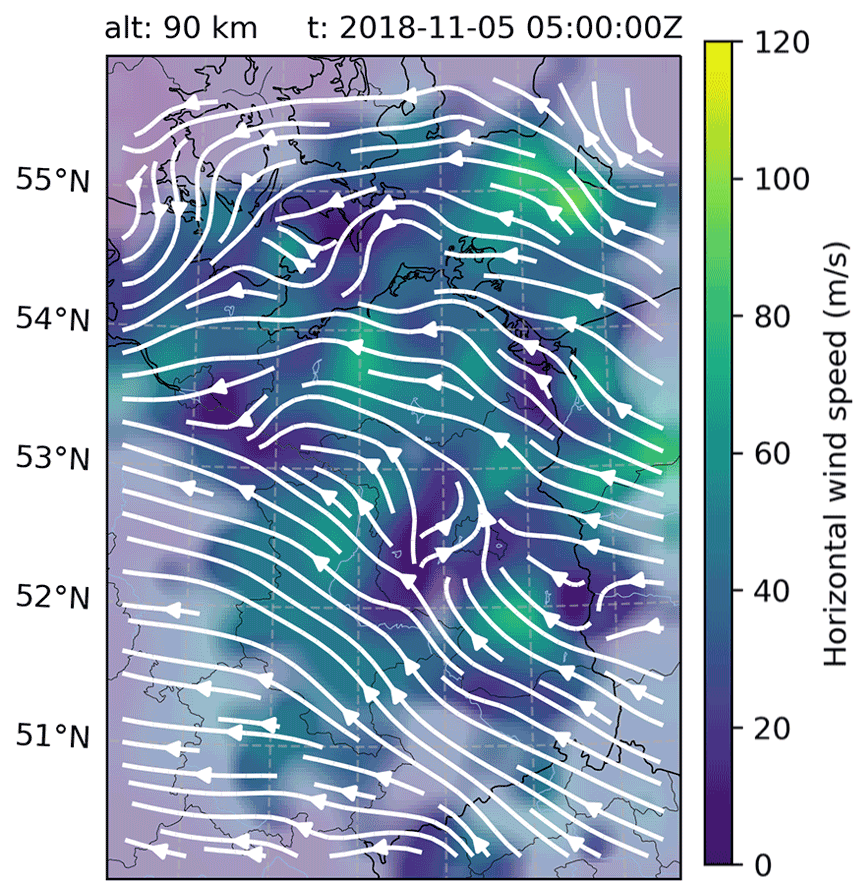
\includegraphics[width=2.5cm]{img/volz_2021.png}
        };
        \node<2-> at (image.center) {%
            \begin{tcolorbox}[width = 2cm, center, boxrule=0pt,colback=yellow,arc=0pt,auto outer arc,left=0pt,right=0pt,boxsep=0pt]
                \centering
                \footnotesize
                Wind maps
            \end{tcolorbox}
        };
        \node<2->[anchor=south east] at ([yshift=0cm, xshift=-0.5cm]image.south east) {%
            {\fontsize{3}{3.4}\selectfont \textcolor{white}{Credit: \citeauthor{volz_FourdimensionalMesosphericLower_2021}, \citeyear{volz_FourdimensionalMesosphericLower_2021} \cite{volz_FourdimensionalMesosphericLower_2021}}}
        };
        \node<2->[anchor=south east] (image) at ([xshift=-3.5cm - 5pt, yshift=0.5cm]current page.south east) {
            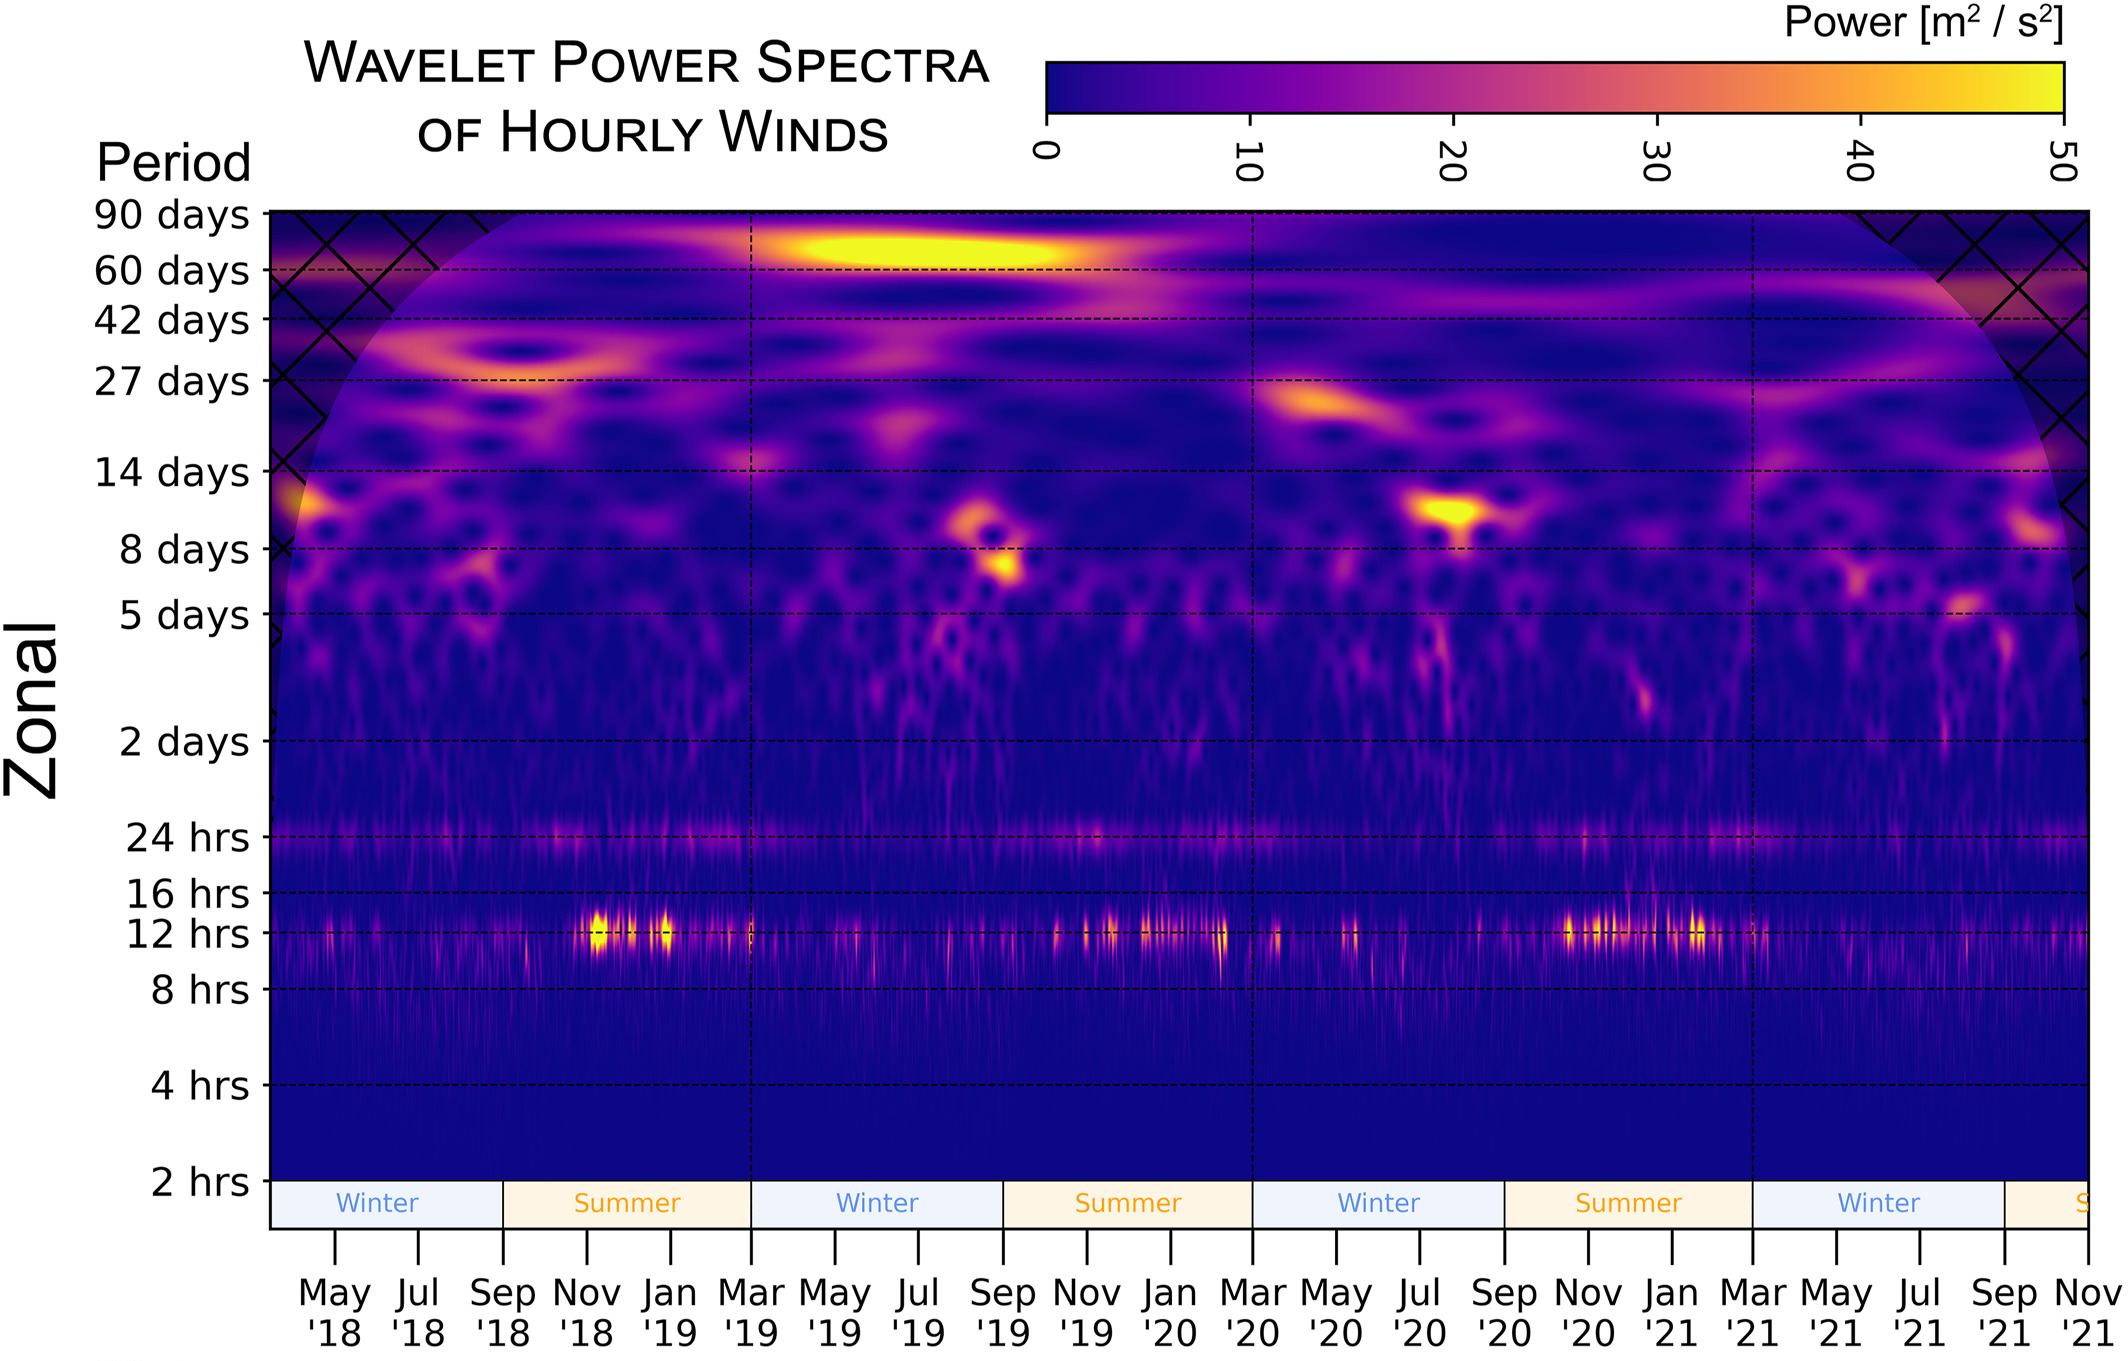
\includegraphics[width=5cm]{img/mcmurdo_wavelet.png}
        };
        \node<2-> at ([xshift=0.25cm, yshift=0.5cm]image.center) {%
            \begin{tcolorbox}[width = 3cm, center, boxrule=0pt,colback=yellow,arc=0pt,auto outer arc,left=0pt,right=0pt,boxsep=0pt]
                \centering
                \footnotesize
                Atmospheric tide temporal analysis
            \end{tcolorbox}
        };
        \node<2->[anchor=south east] at ([yshift=0.5cm, xshift=-0.1cm]image.south east) {%
            {\fontsize{3}{3.4}\selectfont \textcolor{white}{Credit: \citeauthor{marino_FirstObservationsNew_2022}, \citeyear{marino_FirstObservationsNew_2022} \cite{marino_FirstObservationsNew_2022}}}
        };
        \node<2->[anchor=south east] (image) at ([xshift=0cm, yshift=0.5cm]current page.south east) {
                \adjincludegraphics[width=3.5cm,trim={{.5\width} 0  0 {.12\height}},clip]{img/12h_z_90pm2km_15d_results.pdf}};
        \node<2-> at (image.center) {%
            \begin{tcolorbox}[width = 3cm, center, boxrule=0pt,colback=yellow,arc=0pt,auto outer arc,left=0pt,right=0pt,boxsep=0pt]
                \centering
                \footnotesize
                Atmospheric tide spatial analysis
            \end{tcolorbox}
        };
        \node<2->[anchor=south east] (image) at ([xshift=0cm, yshift=0.5cm + 4.5cm + 5pt]current page.south east) {
            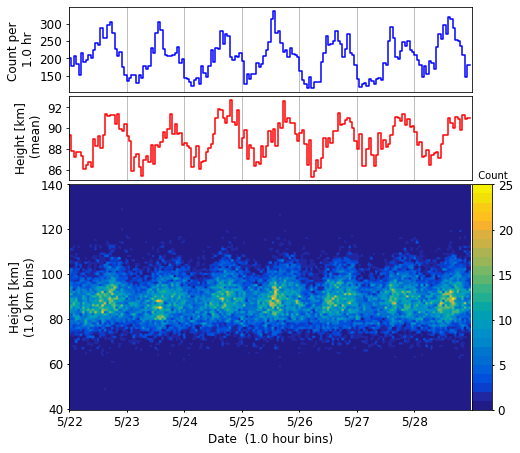
\includegraphics[width=3.5cm]{img/meteor_stats.png}
        };
        \node<2-> at (image.center) {%
            \begin{tcolorbox}[width = 3cm, center, boxrule=0pt,colback=yellow,arc=0pt,auto outer arc,left=0pt,right=0pt,boxsep=0pt]
                \centering
                \footnotesize
                Meteor statistics
            \end{tcolorbox}
        };
        \node<2-> at ([xshift=-3.25cm, yshift=-0.5cm]image.center) {%
            \begin{tcolorbox}[width = 2cm, center, boxrule=0pt,colback=yellow,arc=0pt,auto outer arc,left=0pt,right=0pt,boxsep=0pt]
                \centering
                \footnotesize
                \textit{...and more!}
            \end{tcolorbox}
        };
    \end{tikzpicture}
\end{frame}

\begin{frame}[label=zoverview]
    \frametitle{Zephyr Meteor Radar Network}
    \begin{columns}
        \begin{column}{0.6\textwidth}
            The \alert{Zephyr meteor radar network} is our lab's multistatic network, established late 2021.
            \begin{itemize}
                \item \(1\times\) interferometric \textcolor{blue}{\textbf{TX}} array in Boulder, CO
                \item \(4 \times\) \textcolor{red}{\textbf{RX}} throughout CO
                \item Fully polarimetric links
            \end{itemize}
        \end{column}
        \begin{column}{0.25\textwidth}
            \centering %
            {\linespread{1}\tiny %
            \centering%
            \begin{tabular}{R{1.5cm} m{1.1cm}}
                \hline
                \rowcolor[HTML]{C0C0C0} 
                \textbf{Parameter}                   & \textbf{Value}         \\ \hline
                Frequency:                   & 31.25 MHz     \\
                \textcolor{blue}{\textbf{TX}} bandwidth: & 200 kHz       \\
                Channel power:               & 500 W         \\
                Channels:             & 6             \\
                Code length:                 & 1,000 Chips   \\
                Chip duration:               & 5 \(\mu s\)   \\
                Chip length:            & 1.5 km  \\
                \hline
            \end{tabular}}%
        \end{column}
        \begin{column}{0.22\textwidth}
            \centering
            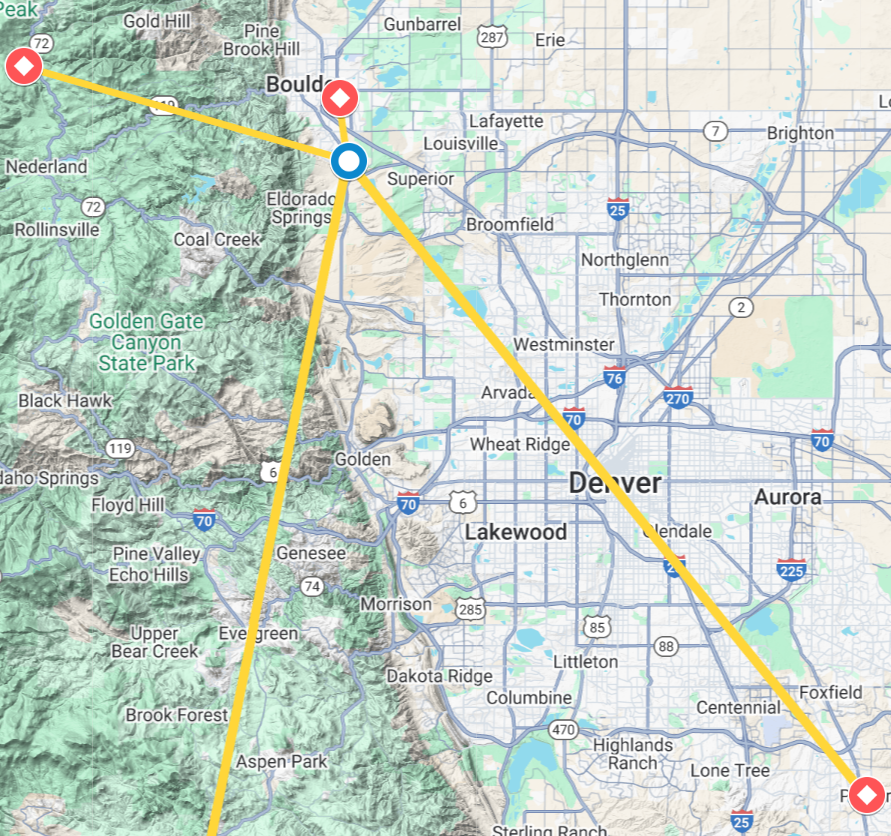
\includegraphics[width=\linewidth]{img/zephyr_map.png}
        \end{column}%
    \end{columns}%
    \centering
    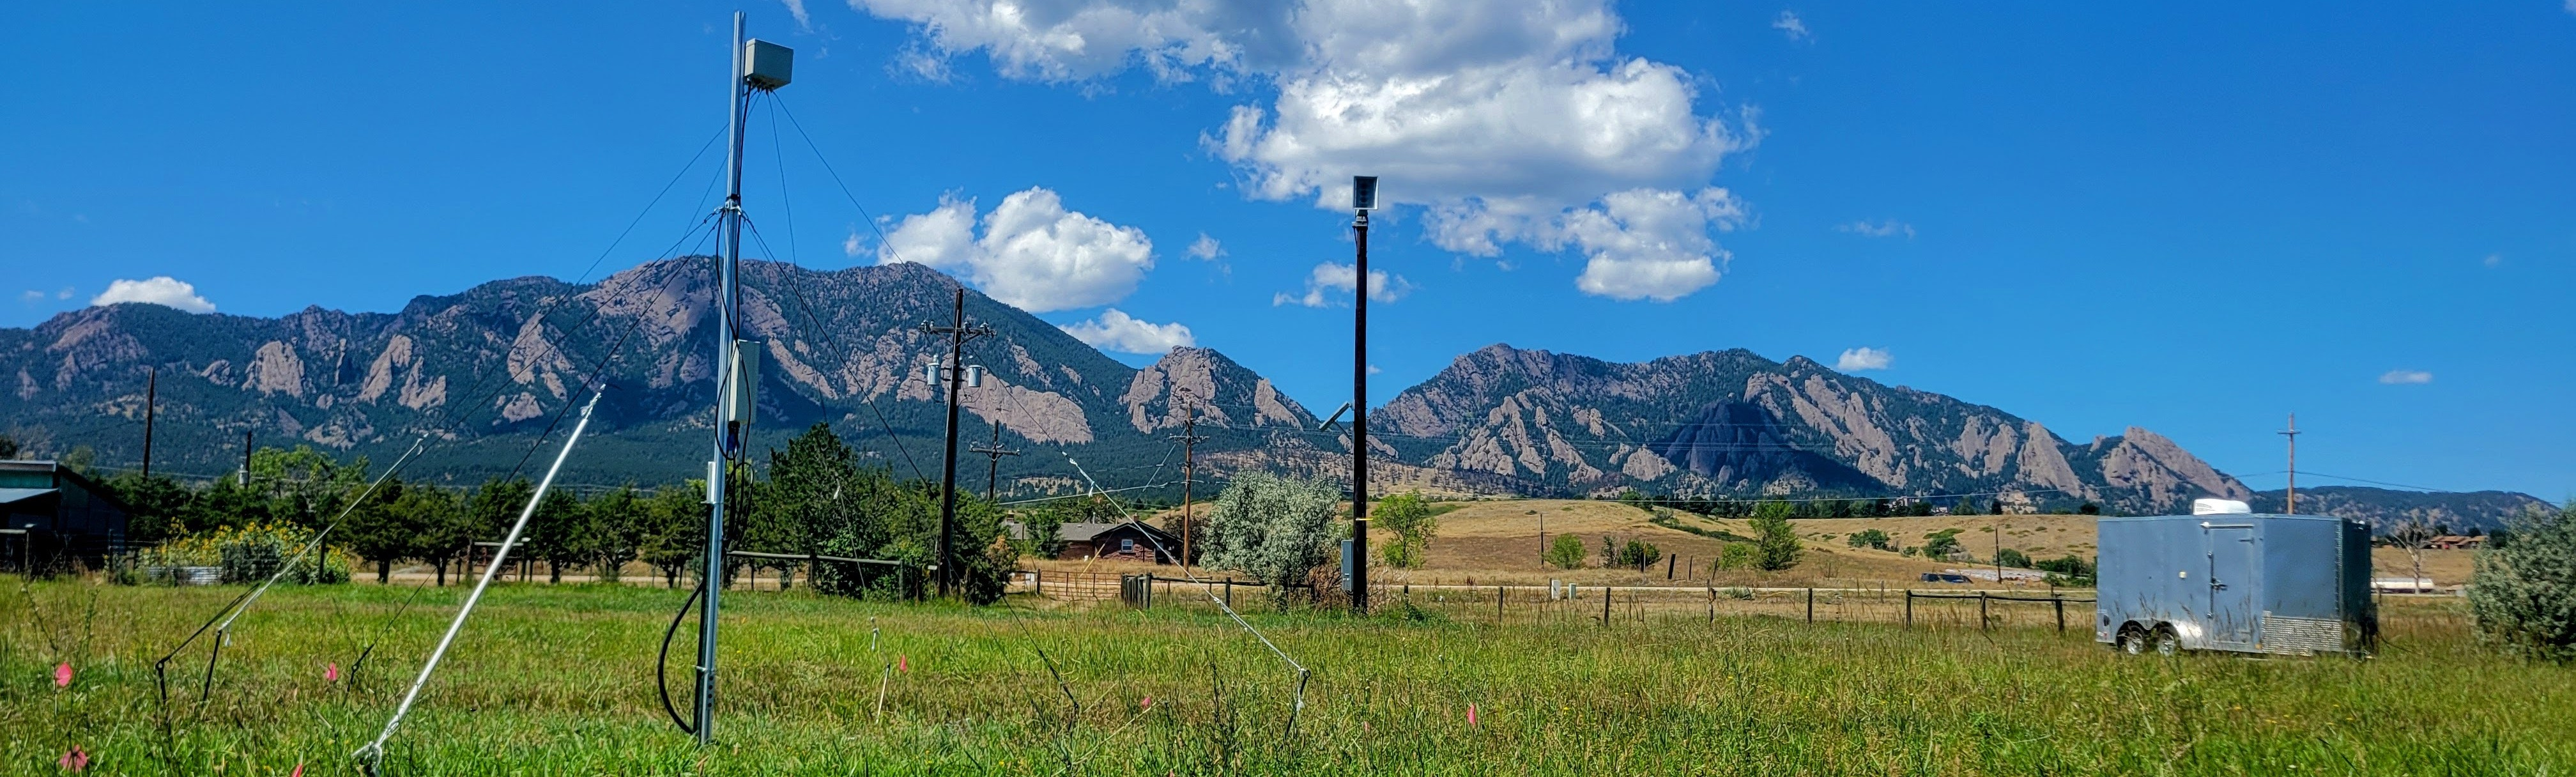
\includegraphics[width=\linewidth]{img/zephyr.jpg}
\end{frame}


\section[Current Positioning Standard: Interferometry]{Interferometry}

\begin{frame}[label=IF_basis]
    \frametitle{How Do We Locate Meteors?}
    \begin{columns}
        \begin{column}{0.6\textwidth}
            Through \alert{interferometry}:
            {\setlength{\leftmargini}{1em} %
            \begin{enumerate} \footnotesize
                \item<+-> Each \textcolor{blue}{\textbf{TX}} antenna sends out a unique signal
                \item<+-> Each signal takes slightly different paths
                % \begin{itemize}
                    % \item The signal whose antenna is closest to the meteor will arrive first
                    % \item The signal whose antenna is furthest to the meteor will arrive last 
                    % \item[\(\blacktriangleright\)] Each antenna is a different distance from the meteor
                    % \item[\(\blacktriangleright\)] {Each point in the sky will have a unique(ish) set of signal delays}
                    % \item E.g., for a meteor directly north of the array: the north antenna's signal will arrive before the south antenna's signal 
                % \end{itemize} 
                \item<+-> Signals bounce off the meteor trail towards \textcolor{red}{\textbf{RX}}
                \item<+-> \textcolor{red}{\textbf{RX}} measures each signal's phase
                \item<+-> Math is used to find the direction of arrival that best fits the signals' relative phases
            \end{enumerate}}
        \end{column}
        \begin{column}{0.5\textwidth}
            \centering
            \begin{tikzpicture}
                \node[anchor=south west, inner sep=0] (image) at (0,0) {%
                    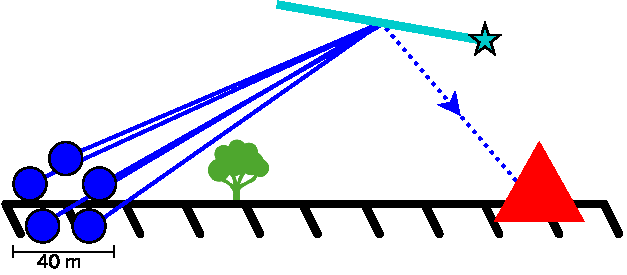
\includegraphics[width=\linewidth]{img/IF_basis.pdf}
                };
                \node<1->[circle, draw=yellow, fill=yellow!30, thick, minimum size=1mm] 
                at ([xshift=-2cm, yshift=0cm]image.center) {\scriptsize 1};
                \uncover<2->{\node[circle, draw=yellow, fill=yellow!30, thick, minimum size=1mm] 
                at ([xshift=0.8cm, yshift=0.2cm]image.north) {\scriptsize  2};}
                \uncover<3->{\node[circle, draw=yellow, fill=yellow!30, thick, minimum size=1mm] 
                at ([xshift=1.25cm, yshift=0cm]image.center) {\scriptsize  3};}
                \uncover<4->{\node[circle, draw=yellow, fill=yellow!30, thick, minimum size=1mm] 
                at ([xshift=-0.25cm, yshift=1cm]image.south east) {\scriptsize 4};}
                \uncover<5->{\node[circle, draw=yellow, fill=yellow!30, thick, minimum size=1mm] 
                (five) at ([xshift=-0.25cm, yshift=-0.5cm]image.south east) {\scriptsize 5};}
                \uncover<5->{\node[anchor = east] at ([xshift=0.1cm]five.west) { 
                    \uncovergraphics<5->[width=0.75cm]{img/calc.pdf}
                };}
        \end{tikzpicture}
        \end{column}
    \end{columns}
    \centering \uncover<6->{\hl{\textbf{Each point in the sky will have a unique* set of signal delays}}} \\ ~ \\

    \uncover<6->{\tiny *\textit{with a high SNR, good array geometry, and a well-calibrated link}}
\end{frame}

% \begin{frame}[label=ears]
    \frametitle{Analogy: Ears as Interferometric Arrays}
    You locate sounds by comparing what each ear hears:  
    \begin{columns}
        \begin{column}{0.2\textwidth}
            \small \textit{A sound from your right hits your right ear first}
        \end{column}
        \begin{column}{0.4\textwidth}
            \centering
            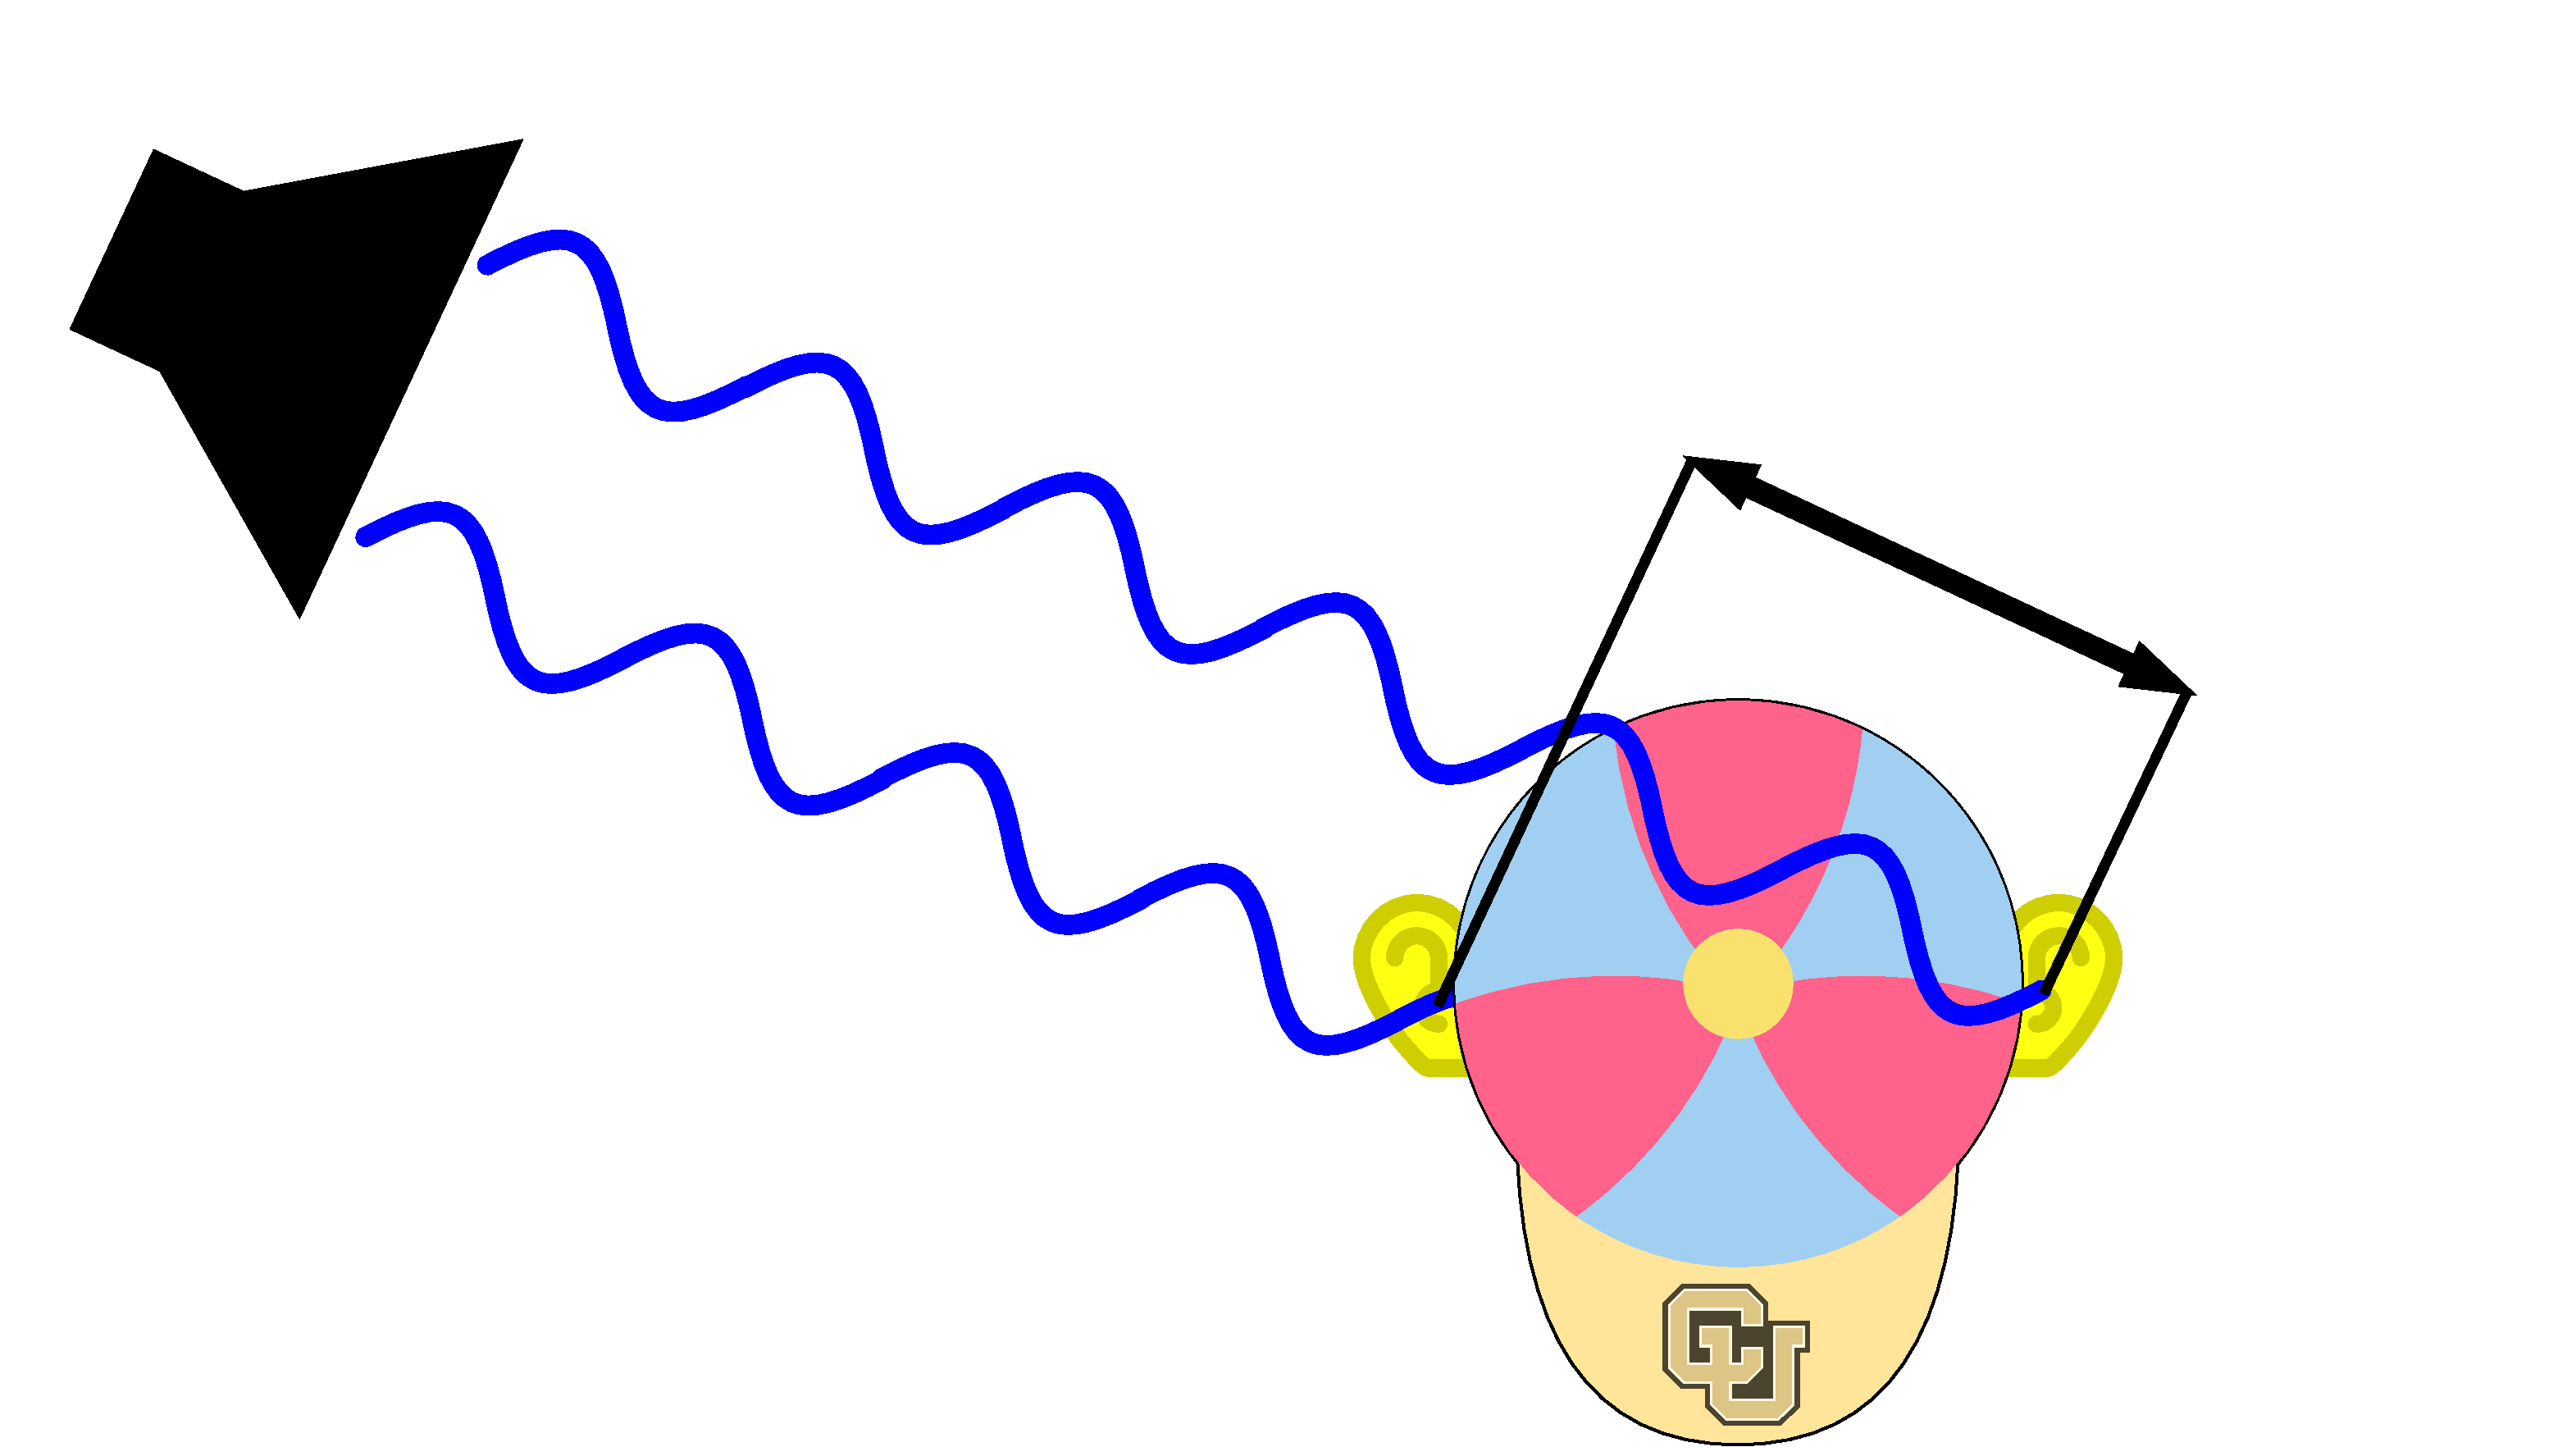
\includegraphics[scale=0.1]{img/ears_left.pdf}
        \end{column}
        \begin{column}{0.2\textwidth}
            \centering
            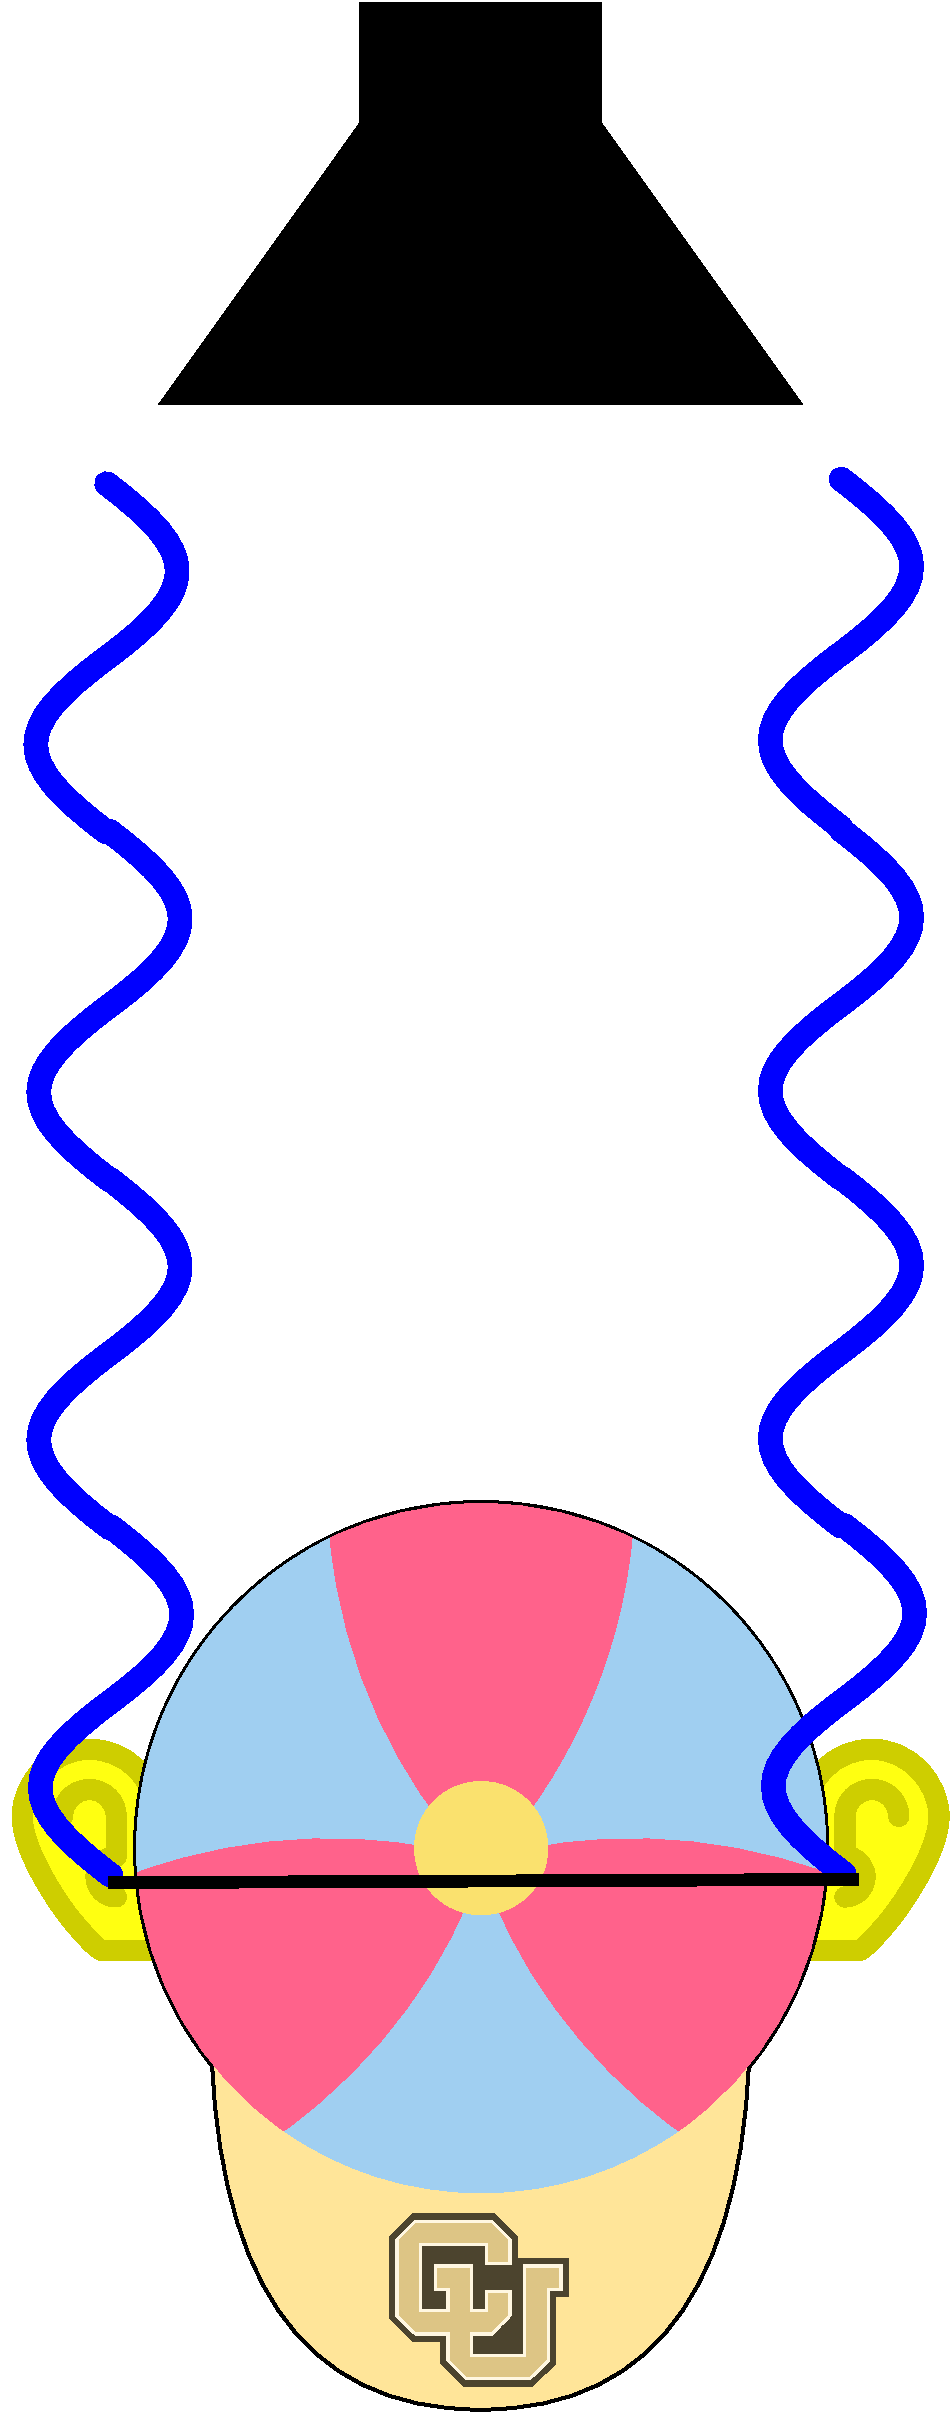
\includegraphics[scale=0.1]{img/ears_behind.pdf}
        \end{column}
        \begin{column}{0.2\textwidth}
            \small \textit{A sound from behind arrives at both ears simultaneously}
        \end{column}
    \end{columns}

    This is analogous to interferometry! 
\end{frame}


\begin{frame}[label=IF_sucks]
    \frametitle{Challenges of Interferometry}
    \begin{columns}
        \begin{column}{0.7\textwidth}
            Requirements:
            \begin{itemize}
                \item \alert{Precise array positioning}
                \item Tedious \alert{calibration} of {every} link
                \item Periodic \alert{re-calibration}  
            \end{itemize}

            Other drawbacks: 
            \begin{itemize}
                \item Positional \alert{uncertainties are difficult} to estimate
                \item Performance drops off or fails low at SNRs, so these \alert{observations are discarded}
            \end{itemize}
            \centering
            \begin{tcolorbox}[width = 0.8\linewidth, center, boxrule=0pt,colback=yellow,arc=0pt,outer arc = 0pt,left=0pt,right=0pt,boxsep=2pt]
            \centering
            \textbf{Interferometry makes deployment, operation, and analysis difficult!}
        \end{tcolorbox}
        \end{column}
        \begin{column}{0.3\textwidth}
            \centering
            \begin{tikzpicture}
                \node[anchor=center, inner sep=0] (img) at (0,0) {
                    {{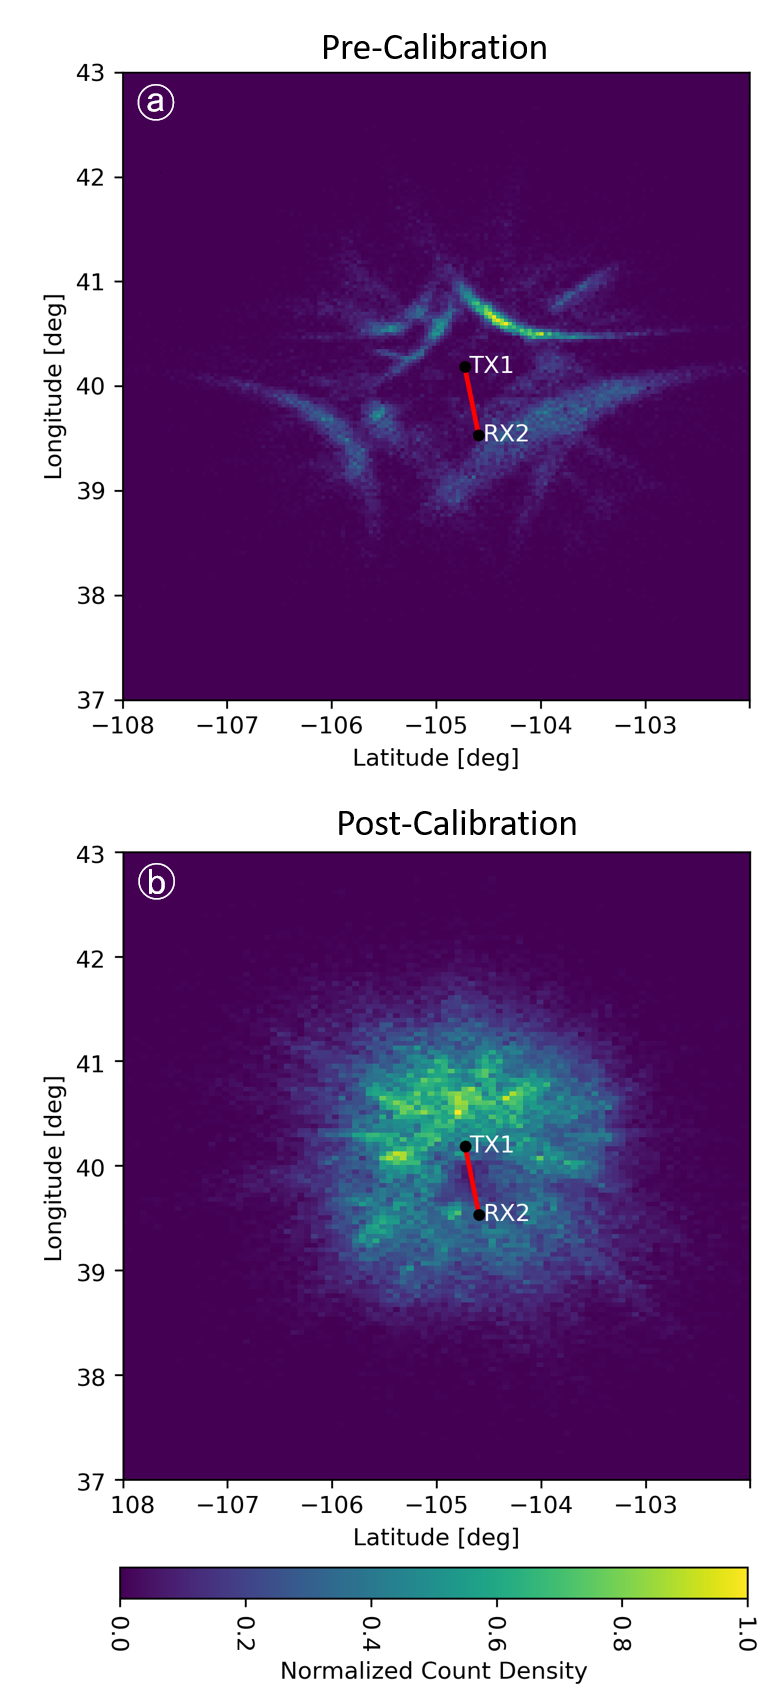
\includegraphics[height=\textheight - 1.5cm]{img/calibration_vert.png}}}
                };
                \node[anchor=north east, inner sep=2pt] at ([yshift=-0.3cm]img.north east) { 
                    {{{\fontsize{3}{3.4}\selectfont\raggedleft \textcolor{white}{\textit{Credit:} \citeauthor{marino_MeteorRadarPhase_2024}, \citeyear{marino_MeteorRadarPhase_2024} \cite{marino_MeteorRadarPhase_2024}}}}}
                };
            \end{tikzpicture}
        \end{column}
    \end{columns}
\end{frame}

\section[Time-of-Flight Position Estimation of Specular Reflection Point]{TOF Position Estimation}

\begin{frame}[label=gps_intro]
    \frametitle{Looking at GNSS}
    \alert{Global navigation satellite systems} (GNSS) have solved these problems!
    \begin{columns}
        \begin{column}{0.5\textwidth}
            Utilizes a \alert{time-of-flight} (TOF) position solution
            \begin{itemize}
                \item Uses only range measurements
                \item Similar signal structure to meteor radar
                \item Provides \alert{easily derived uncertainties}
                \item \alert{Robust} at low SNRs
                \item \alert{No calibration required!}
            \end{itemize}
        \end{column}
        \begin{column}{0.5\textwidth}
            \begin{tikzpicture}
                \node[anchor=center, inner sep=0] (img) at (0,0) {
                    {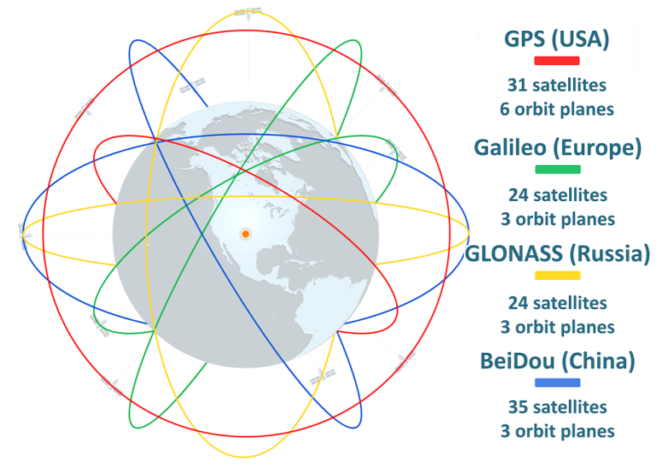
\includegraphics[width=\linewidth]{img/GNSS.png}}
                };
                \node[anchor=south east, inner sep=2pt] at (img.south east) { 
                    {{{\fontsize{3}{3.4}\selectfont\raggedleft \textcolor{black}{\textit{Credit:} \citeauthor{ramadan_HowDoesGNSS_} \cite{ramadan_HowDoesGNSS_}}}}}
                };
            \end{tikzpicture}
        \end{column}
    \end{columns}
\end{frame}

 

\begin{frame}[label=gps_basis]
    \frametitle{GNSS: Basis of Operation}
    Each range measurement gives more information 
    \begin{columns}
        \begin{column}{0.6\textwidth}
            % \begin{itemize} \scriptsize
            %     \item Ranges measured from satellites with known position
            %     \item 4+ range measurements required for user position
            %     \item More measurements \(\xrightarrow[]{}\) more precision
            % \end{itemize}

            Using 4 satellites \(\bullet, \textcolor{cyan}{\bullet}, \textcolor{yellow}{\bullet}, \textcolor{magenta}{\bullet}\):
            {\setlength{\leftmargini}{1em} \begin{itemize} \footnotesize
                \item<2->[\(\blacktriangleright\)] 1 range measurement constrains position to a \alert{sphere} 
                \item<3->[\textcolor{cyan}{\(\blacktriangleright\)}] 2 measurements \(\xrightarrow[]{}\) \alert{circle} 
                \item<4->[\textcolor{green}{\(\blacktriangleright\)}] 3 measurements\(\xrightarrow[]{}\) \alert{2 points}
                \item<5->[\(\vartriangleright \)] 4 measurements \(\xrightarrow[]{}\) \alert{1 point}!
            \end{itemize}}
            \centering
            \uncover<6->{\begin{tcolorbox}[width = 0.6\linewidth, center, boxrule=0pt,colback=yellow,arc=0pt, outer arc=0pt,left=0pt,right=0pt,boxsep=0pt]
                \centering
                \textbf{How can this be adapted for meteor radar?}
            \end{tcolorbox}}
        \end{column}
        \begin{column}{0.4\textwidth}
            \centering %
            \includegraphics<1>[height=0.8\textheight]{img/0spheres.pdf}%
            \includegraphics<2>[height=0.8\textheight]{img/1spheres.pdf}%
            \includegraphics<3>[height=0.8\textheight]{img/2spheres.pdf}%
            \includegraphics<4>[height=0.8\textheight]{img/3spheres.pdf}%
            \includegraphics<5->[height=0.8\textheight]{img/4spheres.pdf}%
        \end{column}
    \end{columns}
\end{frame}

 

\begin{frame}[label=adapting_gps]
    \frametitle{Adapting GNSS Position Solution for Meteor Radar}
    \begin{columns}
        \begin{column}{0.5\textwidth}
            Meteor radar gives \alert{bistatic range measurements} %
            \begin{itemize} \footnotesize %
                \item Distance from \textcolor{blue}{\textbf{TX}}, to meteor trail, to \textcolor{red}{\textbf{RX}}
            \end{itemize}

            % Each measurement constrains the meteor to an \alert{ellipsoid}
            % \begin{itemize} \footnotesize
            %     \item Foci: \textcolor{blue}{\textbf{TX}}, \textcolor{red}{\textbf{RX}}
            %     \item Major axis = bistatic range
            % \end{itemize}

            Using \textcolor{cyan}{\textbf{RX}\textsubscript{1}}, \textcolor{magenta}{\textbf{RX}\textsubscript{2}}, \textcolor{yellow}{\textbf{RX}\textsubscript{3}}, {\textbf{RX}\textsubscript{4}}:
            {\setlength{\leftmargini}{1em} \begin{itemize} \footnotesize
                \item<2->[\(\blacktriangleright\)] 1 bistatic range measurement constrains position to an \alert{ellipsoid} 
                \item<3->[{\(\blacktriangleright\)}] 2 measurements \(\xrightarrow[]{}\) \alert{ellipse} 
                \item<4->[{\(\blacktriangleright\)}] 3 measurements \(\xrightarrow[]{}\) \alert{2 points}
                \item<5->[\(\blacktriangleright\)] 4 measurements \(\xrightarrow[]{}\) \alert{1 point}!
            \end{itemize}}
        \end{column}
        \begin{column}{0.6\textwidth}
            \begin{tikzpicture}[remember picture,overlay]
                \node<1>[anchor=east] at ([yshift=-0.35cm]current page.east) {
                    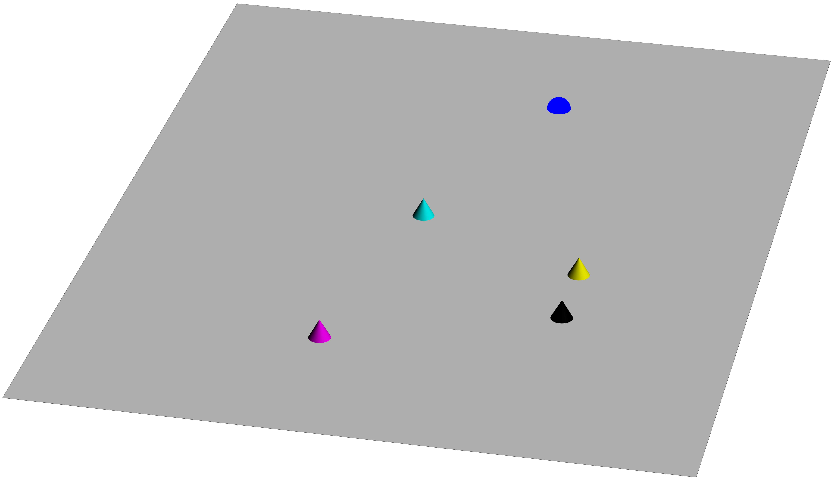
\includegraphics[width=\linewidth]{img/0ellipsoids.pdf}%
                };
                \node<2>[anchor=east] at (current page.east) {
                    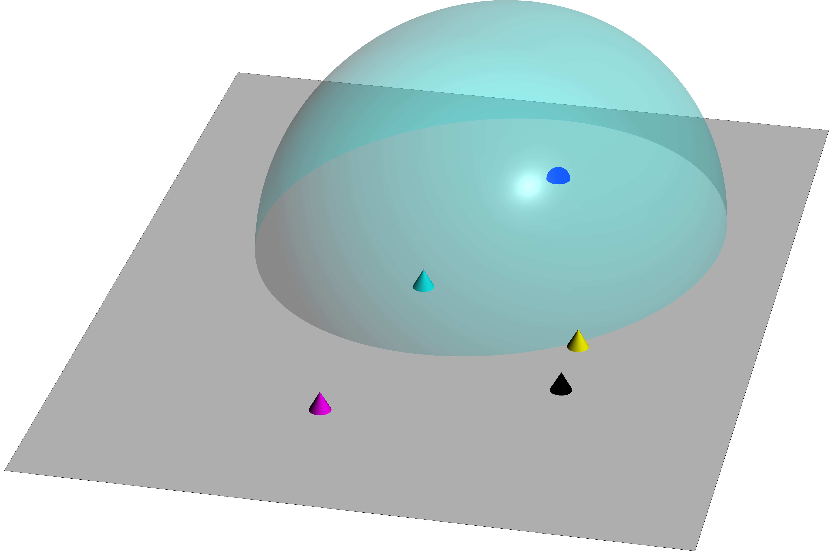
\includegraphics[width=\linewidth]{img/1ellipsoids.pdf}%
                };
                \node<3>[anchor=east] at (current page.east) {
                    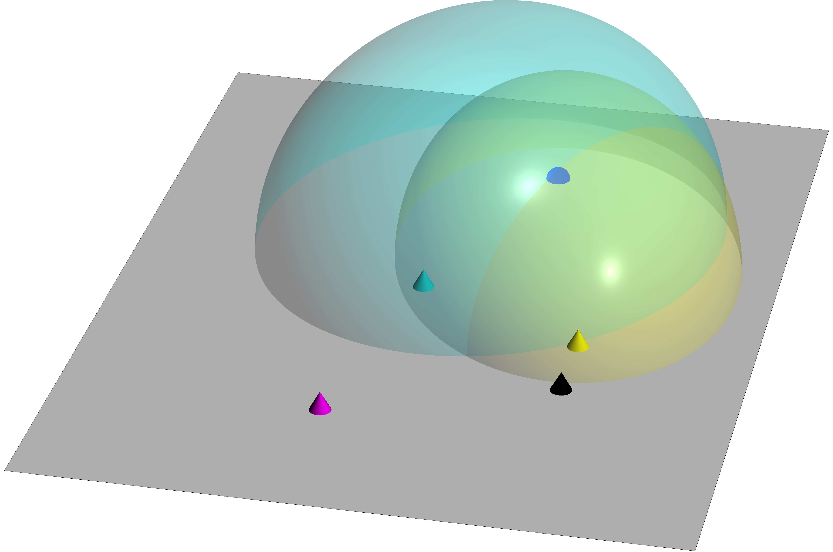
\includegraphics[width=\linewidth]{img/2ellipsoids.pdf}%
                };
                \node<4>[anchor=east] at (current page.east) {
                    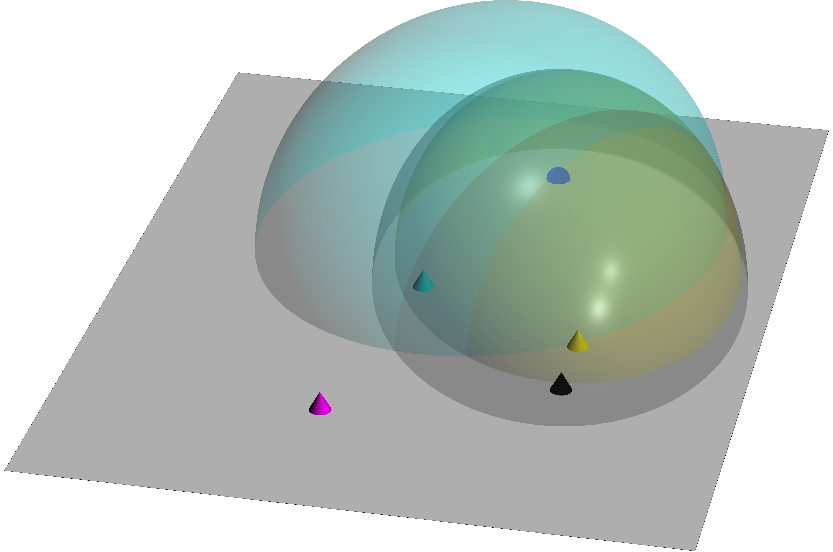
\includegraphics[width=\linewidth]{img/3ellipsoids.pdf}%
                };
                \node<5->[anchor=east] at ([yshift=-0.15cm]current page.east) {
                    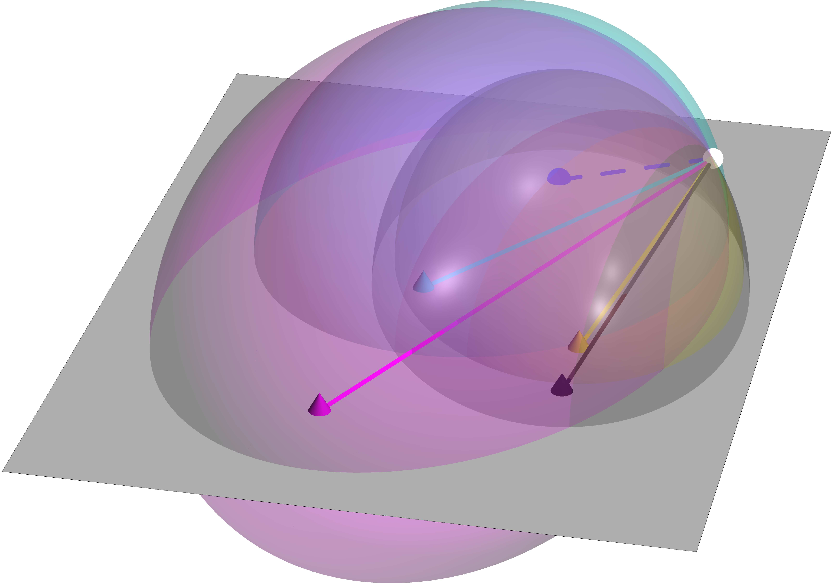
\includegraphics[width=\linewidth]{img/4ellipsoids.pdf}%
                };
            \end{tikzpicture}
        \end{column}
    \end{columns}
\end{frame} 

\begin{frame}[t, label=gnss_ls]
    \frametitle{TOF Estimation of Meteor Location}
    \begin{center}
        \textit{\textcolor{red}{Warning}: Math Time!}
    \end{center}
    
    The meteor trail's reflection point can be estimated using \alert{iterative linearized least squares}: 
    \begin{equation*}
        \hat{\mathbf{r}}^s = \left( \mathbf{G}^{\top} \mathbf{G} \right)^{-1} \mathbf{G}^{\top} \left(\boldsymbol{\rho} - \boldsymbol{\rho}(\mathbf{r}^s_0)  \right) + \mathbf{r}_0^s
    \end{equation*}
    \begin{columns}[t]
        \begin{column}{0.1\linewidth}
            Where:
        \end{column}
        \begin{column}{0.3\linewidth}
            {\setlength{\leftmargini}{0em} \begin{itemize} \scriptsize \vspace{-1.5\baselineskip}%
                \item[\(\blacktriangleright\)] \hlonly<2->{{\(\boldsymbol{\rho}\)}: vector of 4+ measured ranges}
                \item[\(\blacktriangleright\)] \hlonly<4->{{\(\hat{\mathbf{r}}^s\)}: estimated reflection point}
                \item[\(\blacktriangleright\)] \(\mathbf{r}^s_0 = [x_0^s, y_0^s, z_0^s]\): linearization point
                \item[\(\blacktriangleright\)] \(\mathbf{r}^T = [x^{T}, y^{T}, z^{T}]\): location of \textcolor{blue}{\textbf{TX}}\textsubscript{j}
                \item[\(\blacktriangleright\)] \(\mathbf{r}^{R_j} = [x^{R_j}, y^{R_j}, z^{R_j}]\): location of \textcolor{red}{\textbf{RX}}
            \end{itemize}}
        \end{column}
        \begin{column}{0.6\linewidth}
            {\setlength{\leftmargini}{0em} \begin{itemize} \scriptsize \vspace{-1.5\baselineskip}%
                \item[\(\blacktriangleright\)] \hlonly<3->{{\(\mathbf{G}\)}: geometry matrix}, relating \textcolor{blue}{\textbf{TX}}/\textcolor{red}{\textbf{RX}}/\(\mathbf{r}^s\) locations to bistatic range
            \end{itemize}} \scriptsize
            \begin{equation*}
                \mathbf{G} = 
                \begin{bmatrix} 
                    \frac{x_{0}^s - x^{R_1}}{|\mathbf{r}_0^s - \mathbf{r}^{R_1}|} +  \frac{x_{0}^s - x^{T}}{|\mathbf{r}_0^s - \mathbf{r}^{T}|} & 
                    \frac{y_{0}^s - y^{R_1}}{|\mathbf{r}_0^s - \mathbf{r}^{R_1}|} +  \frac{y_{0}^s - y^{T}}{|\mathbf{r}_0^s - \mathbf{r}^{T}|} & 
                    \frac{z_{0}^s - z^{R_1}}{|\mathbf{r}_0^s - \mathbf{r}^{R_1}|} +  \frac{z_{0}^s - z^{T}}{|\mathbf{r}_0^s - \mathbf{r}^{T}|}  \\ 
                    \vdots & \vdots & \vdots  \\ 
                    \frac{x_{0}^s - x^{R}}{|\mathbf{r}_0^s - \mathbf{r}^{R_j}|} +  \frac{x_{0}^s - x^{T}}{|\mathbf{r}_0^s - \mathbf{r}^{T}|} & 
                    \frac{y_{0}^s - y^{R_j}}{|\mathbf{r}_0^s - \mathbf{r}^{R_j}|} +  \frac{y_{0}^s - y^{T}}{|\mathbf{r}_0^s - \mathbf{r}^{T}|} & 
                    \frac{z_{0}^s - z^{R_j}}{|\mathbf{r}_0^s - \mathbf{r}^{R_j}|} +  \frac{z_{0}^s - z^{T}}{|\mathbf{r}_0^s - \mathbf{r}^{T}|}  
                \end{bmatrix}
            \end{equation*}
        \end{column}
    \end{columns}
    \textit{Initial guess \(\xrightarrow[]{}\) estimate position \(\xrightarrow[]{}\) update guess \(\xrightarrow[]{}\) repeat until convergence}
\end{frame}  

\begin{frame}[label=gnss_viability]
    \frametitle{TOF Precision depends on \alert{Measurement Errors}}
    % \textit{Position estimate uncertainties depends on...}  (1) \colorbox{yellow}{\textbf{Measurement Errors}}
    \begin{columns}[T]
        \begin{column}{0.5\textwidth}
            Range measurements have uncertainty: %
            \begin{center}
                \(\sigma_\rho = \sqrt{2\sigma^2_{clk} + 2\sigma^2_{pos} + \sigma^2_{\Delta\tau}}\)
            \end{center} %
            {\setlength{\leftmargini}{1em} \begin{itemize}
                \item \(\sigma_{clk} = \qty{3}{\m}\): \textcolor{blue}{\textbf{TX}}/\textcolor{red}{\textbf{RX}} clock instability
                \item \(\sigma_{pos} = \qty{1}{m}\): \textcolor{blue}{\textbf{TX}}/\textcolor{red}{\textbf{RX}} positional uncertainty
                \item \(\sigma_{\Delta\tau} \approx \sqrt{\frac{1}{2 T_{coh} C/N_0}} \): Signal correlation error
                \begin{itemize}
                    \item 8 m typical 
                    \item \(T_{coh}\): Coherent integration time
                    \item \(C/N_0\): Carrier-to-noise ratio
                \end{itemize}
            \end{itemize}}
        \end{column}
        \vrule{}
        \begin{column}{0.5\textwidth}
            \alert{Correlation error}: Meteor trail is \textit{\textbf{not}} a point-like reflector
            \begin{itemize}
                \item Elongated reflector smears echo
                \item Correlation against \textcolor{blue}{\textbf{TX}} waveform \(\xrightarrow[]{}\) positive range bias (\textcolor{green}{\textit{\textbf{green}}})
            \end{itemize}
            \centering
            \begin{tikzpicture}
                    \node[anchor=east, inner sep = 0] (img1) at (0,0) { 
                        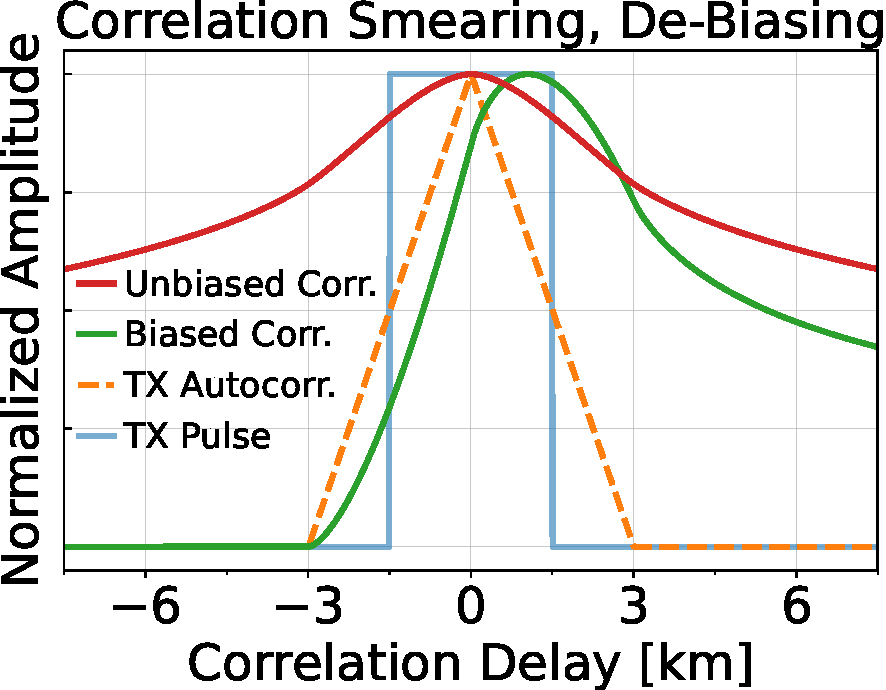
\includegraphics[width=0.55\linewidth]{img/corr_smear_0F1.pdf}
                    };
                    \node[anchor=west, inner sep=0] (img) at (img1.east) {%
                        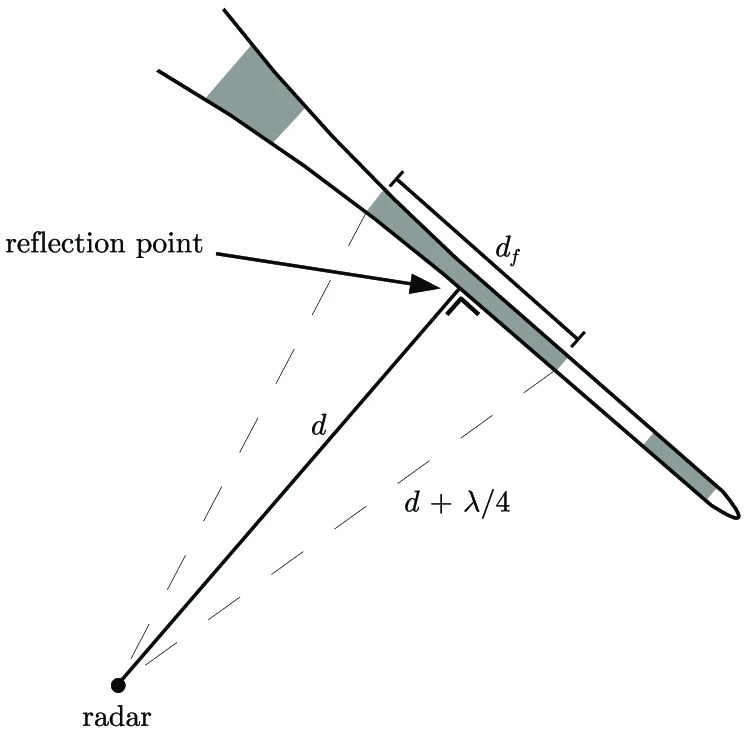
\includegraphics[width=0.4\linewidth]{img/verbeeck_ProceedingsRadioMeteor_2005.png}
                    };
                    \node[anchor=north east, inner sep=2pt] at ([yshift=-0.0cm]img.north east) { 
                    {{{\fontsize{3}{3.4}\selectfont\raggedleft \textcolor{black}{\textit{Credit:} \citeauthor{verbeeck_ProceedingsRadioMeteor_2005}, \citeyear{verbeeck_ProceedingsRadioMeteor_2005} \cite{verbeeck_ProceedingsRadioMeteor_2005}}}}}
                };
            \end{tikzpicture}
        \end{column}
    \end{columns}
    \centering % 
    \alert{De-biased Trail correlation function derived} (\textcolor{red}{\textit{\textbf{red}}})
\end{frame}

\begin{frame}[label=precision_requirements]
    \frametitle{TOF Precision: Propagation and Requirements}
    \begin{columns}
        \begin{column}{0.7\textwidth}
            TOF precision depends on \alert{array geometry}: 
            \begin{center}
                \scriptsize
                \alert{Larger array} \(\xrightarrow[]{}\) More diverse measurements
                
                \(\xrightarrow[]{}\) \alert{smaller positional uncertainties}
            \end{center}

            Quantified through dilution of precision (DOP) matrix: 
            {\scriptsize \begin{equation*} \scriptsize
                \mathbf{H} = \left( \mathbf{G}^{\top} \mathbf{G} \right)^{-1}
            \end{equation*}}
            %
            {Measurement \alert{errors are propagated} to get positional uncertainties: 
            {\scriptsize 
            \begin{align*}
                \begin{matrix}  
                    \sigma_E = \sigma_{\rho} \cdot \sqrt{H_{1,1}}  \qquad \qquad & \sigma_N = \sigma_{\rho} \cdot \sqrt{H_{2,2}} & \qquad \qquad \sigma_U = \sigma_{\rho} \cdot \sqrt{H_{3,3}} 
                \end{matrix}
            \end{align*}}}

            
                \begin{tcolorbox}[width=\linewidth, halign=center,  boxrule=1pt, arc=0pt,auto outer arc,left=0pt,right=0pt,boxsep=0pt]
                Science-driven positional precision requirement:

                \hl{\textbf{1 km uncertainty in altitude}}
            \end{tcolorbox}
        \end{column}
        \begin{column}{0.3\textwidth}
            \begin{tikzpicture}
                \node[anchor=center, inner sep=0] (img) at (0,0) {
                    {{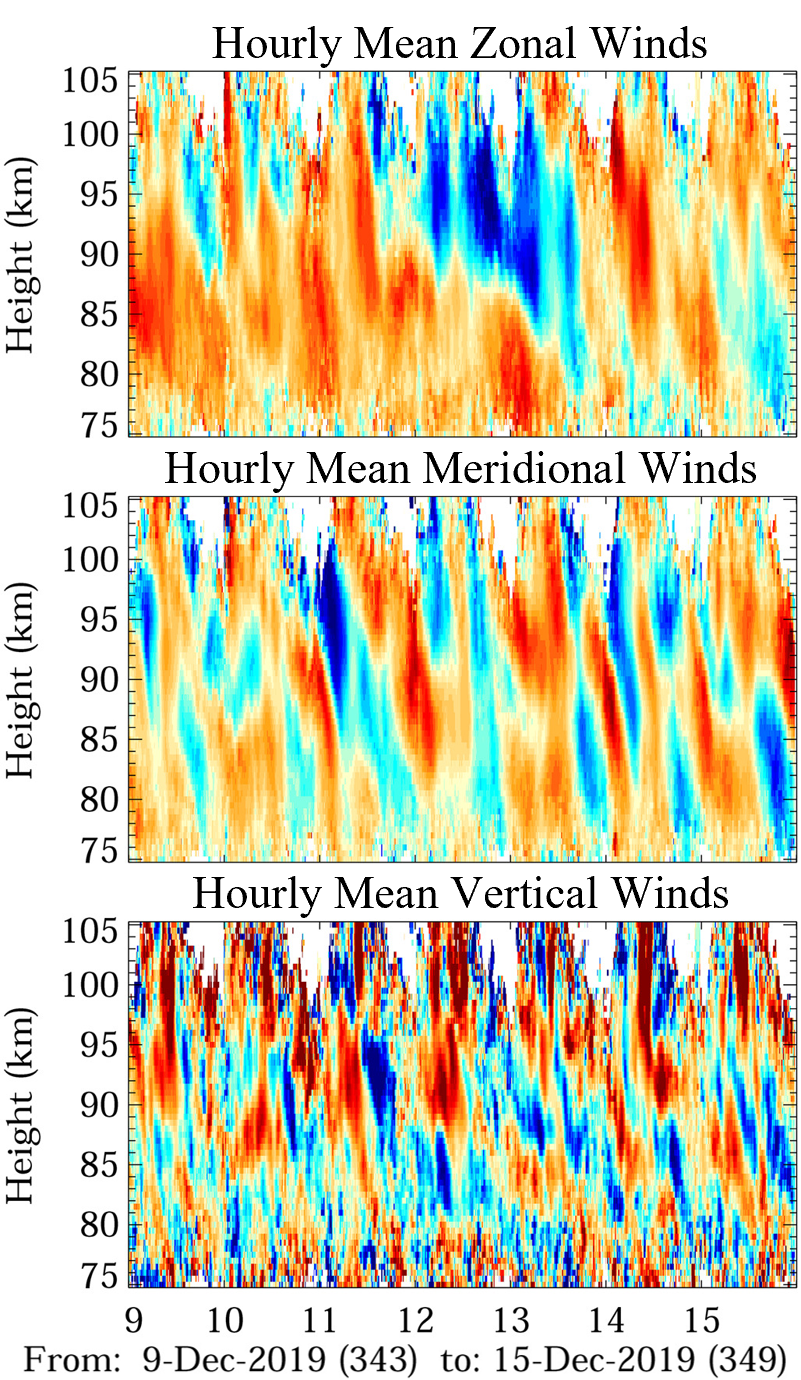
\includegraphics[width=0.7\linewidth]{img/chau_MultistaticSpecularMeteor_2021.png}}}
                };
                \node[anchor=east, inner sep=2pt] at ([yshift=-0.2cm]img.east) { 
                    {{{\fontsize{3}{3.4}\selectfont\raggedleft \textcolor{black}{\textit{Credit:} \citeauthor{chau_MultistaticSpecularMeteor_2021}, \citeyear{chau_MultistaticSpecularMeteor_2021} \cite{chau_MultistaticSpecularMeteor_2021}}}}}
                };
            \end{tikzpicture}        
            {\setlength{\leftmargini}{1em} \begin{itemize} \scriptsize
                \item 2 km altitude bins common
                \item Vertical wavelength of studied dynamics: \(\sim\)10s of km
            \end{itemize}}  
        \end{column}
    \end{columns}
\end{frame}



\begin{frame}[label=change_spec]
    \frametitle{Ensuring Consistent Sampling}

    \begin{columns}
        \begin{column}{0.7\textwidth}
            \textcolor{red}{\textbf{Problem:}} \alert{Reflection point} moves along trail for each \textcolor{red}{\textbf{RX}}
            \begin{itemize} \footnotesize
                \item[\(\blacktriangleright\)] TOF solution assumes reflections from same region 
            \end{itemize}
            \vfill
            \uncover<2->{\textcolor{green}{\textbf{Solution}}: Ensure change in reflection point is small
            \begin{itemize} \footnotesize
                \item[\(\blacktriangleright\)] \(\text{Max. change} = \frac{\text{Max. \textcolor{red}{\textbf{RX}} separation}}{2}\)
                \item All \textcolor{red}{\textbf{RX}} should overlap \alert{Fresnel zones}
            \end{itemize}}

            % \uncover<3->{All \textcolor{red}{\textbf{RX}} should overlap \alert{Fresnel zones}
            % \begin{itemize} \footnotesize
            %     \item[\(\blacktriangleright\)] Region responsible for >90\% of reflected power
            %     \item[\(\blacktriangleright\)] \(\sim 0.7\) km on either side of reflection point
            %     \item[\(\blacktriangleright\)] Overlapping Fresnel zones mean similar spatial sampling
            %     \item[\(\blacktriangleright\)] Solving for \alert{average reflection point} of array
            % \end{itemize} }
        \end{column}
        \begin{column}{0.4\textwidth}
            \centering
            \alt<1-3>{%
                \includegraphics[width=\linewidth]{img/change_in_spec.png}%
            }{%
                \includegraphics[width=\linewidth]{img/change_in_spec_small.png}%
            }
        \end{column}
    \end{columns}
    \begin{columns}[T]
        \begin{column}{0.75\textwidth}
            \alert{Does each \textcolor{red}{\textbf{RX}} in an array reflect off the same region?} 
        \end{column}
        \begin{column}{0.35\textwidth}
            \uncover<4
            >{\hl{\textbf{YES!*}}

            \footnotesize *If the array is not too large...}           
        \end{column}
    \end{columns}
\end{frame}

\begin{frame}
    \frametitle{Conflicting Design Criteria}
    Requirement 1: \alert{1 km positional uncertainty in altitude}
    \begin{itemize}
        \item[\(\blacktriangleright\)] A larger array gives more precise position estimates 
    \end{itemize}


    \uncover<2->{Requirement 2: \alert{\(>50\%\) overlap of Fresnel zones for most observations}
    \begin{itemize}
        \item[\(\blacktriangleright\)] A smaller array gives more consistent spatial sampling
    \end{itemize}}
    \centering
    \uncover<3->{\hl{\textbf{Is there an array size that meets both requirements?}}}
\end{frame}

\section[Results with Monte Carlo Simulation]{Results}

\begin{frame}[label=precision]
    \frametitle{Results: Precision}
    \begin{center}
        {\colorbox{yellow}{\textbf{TOF meets precision requirements for most observations}}}
        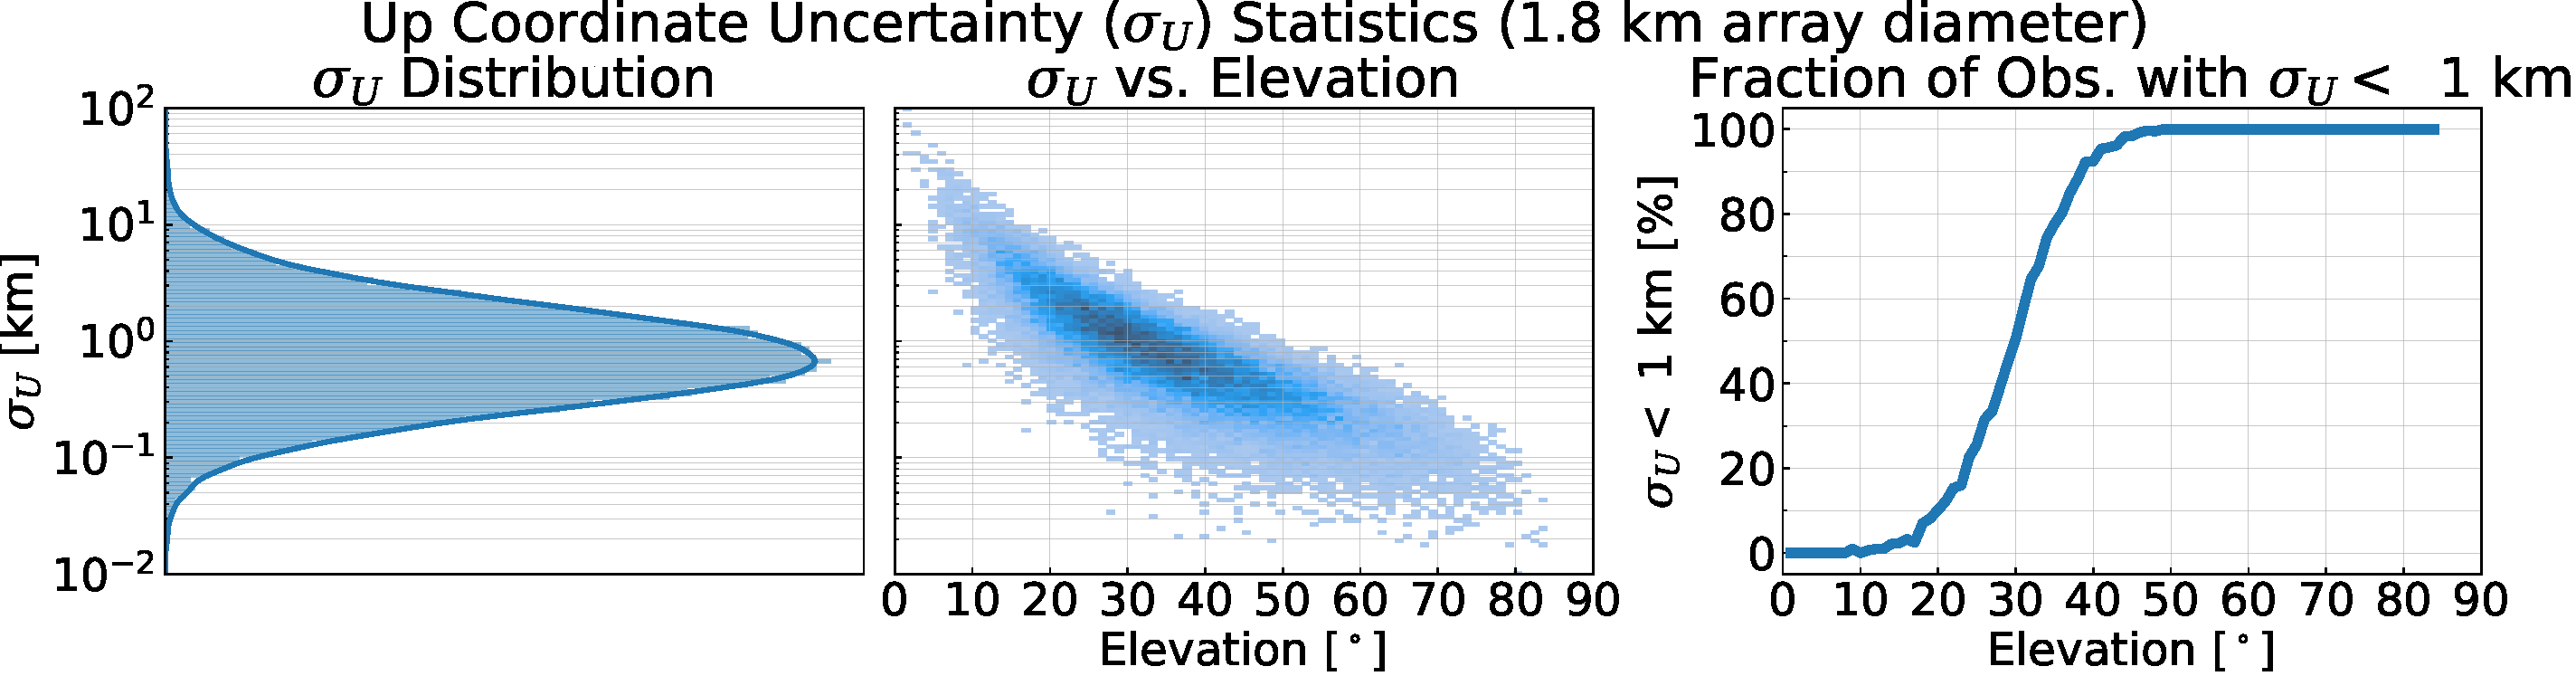
\includegraphics[width=0.8\linewidth]{img/uncert_stats.pdf}
        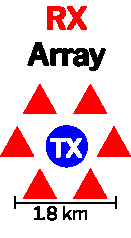
\includegraphics[height=0.35\textheight]{img/rx_array.pdf}
    \end{center}
    \begin{itemize}
        \item[$\blacktriangleright$] \alert{87\% of all high elevation observations} (\(>30^\circ\)) meet requirements
        \begin{itemize}
            \item Average UP uncertainty: 0.56 km 
        \end{itemize}
        \item[$\blacktriangleright$] \alert{48\% of observations at 30\(^\circ\) elevation} meet requirements
        \begin{itemize}
            \item Average UP uncertainty: 1.09 km 
        \end{itemize}
        \item[$\blacktriangleright$] \alert{62\% of all observations} meet requirements
        \item[$\blacktriangleright$] \alert{Average UP uncertainty of 7.17 km}
    \end{itemize}
\end{frame}

\begin{frame}[label=overlap_stats]
    \frametitle{Results: Consistent Sampling}
    \begin{center}
        {\colorbox{yellow}{\textbf{Having all \textcolor{red}{\textbf{RX}} within 1.8 km ensures consistent spatial sampling}}}
        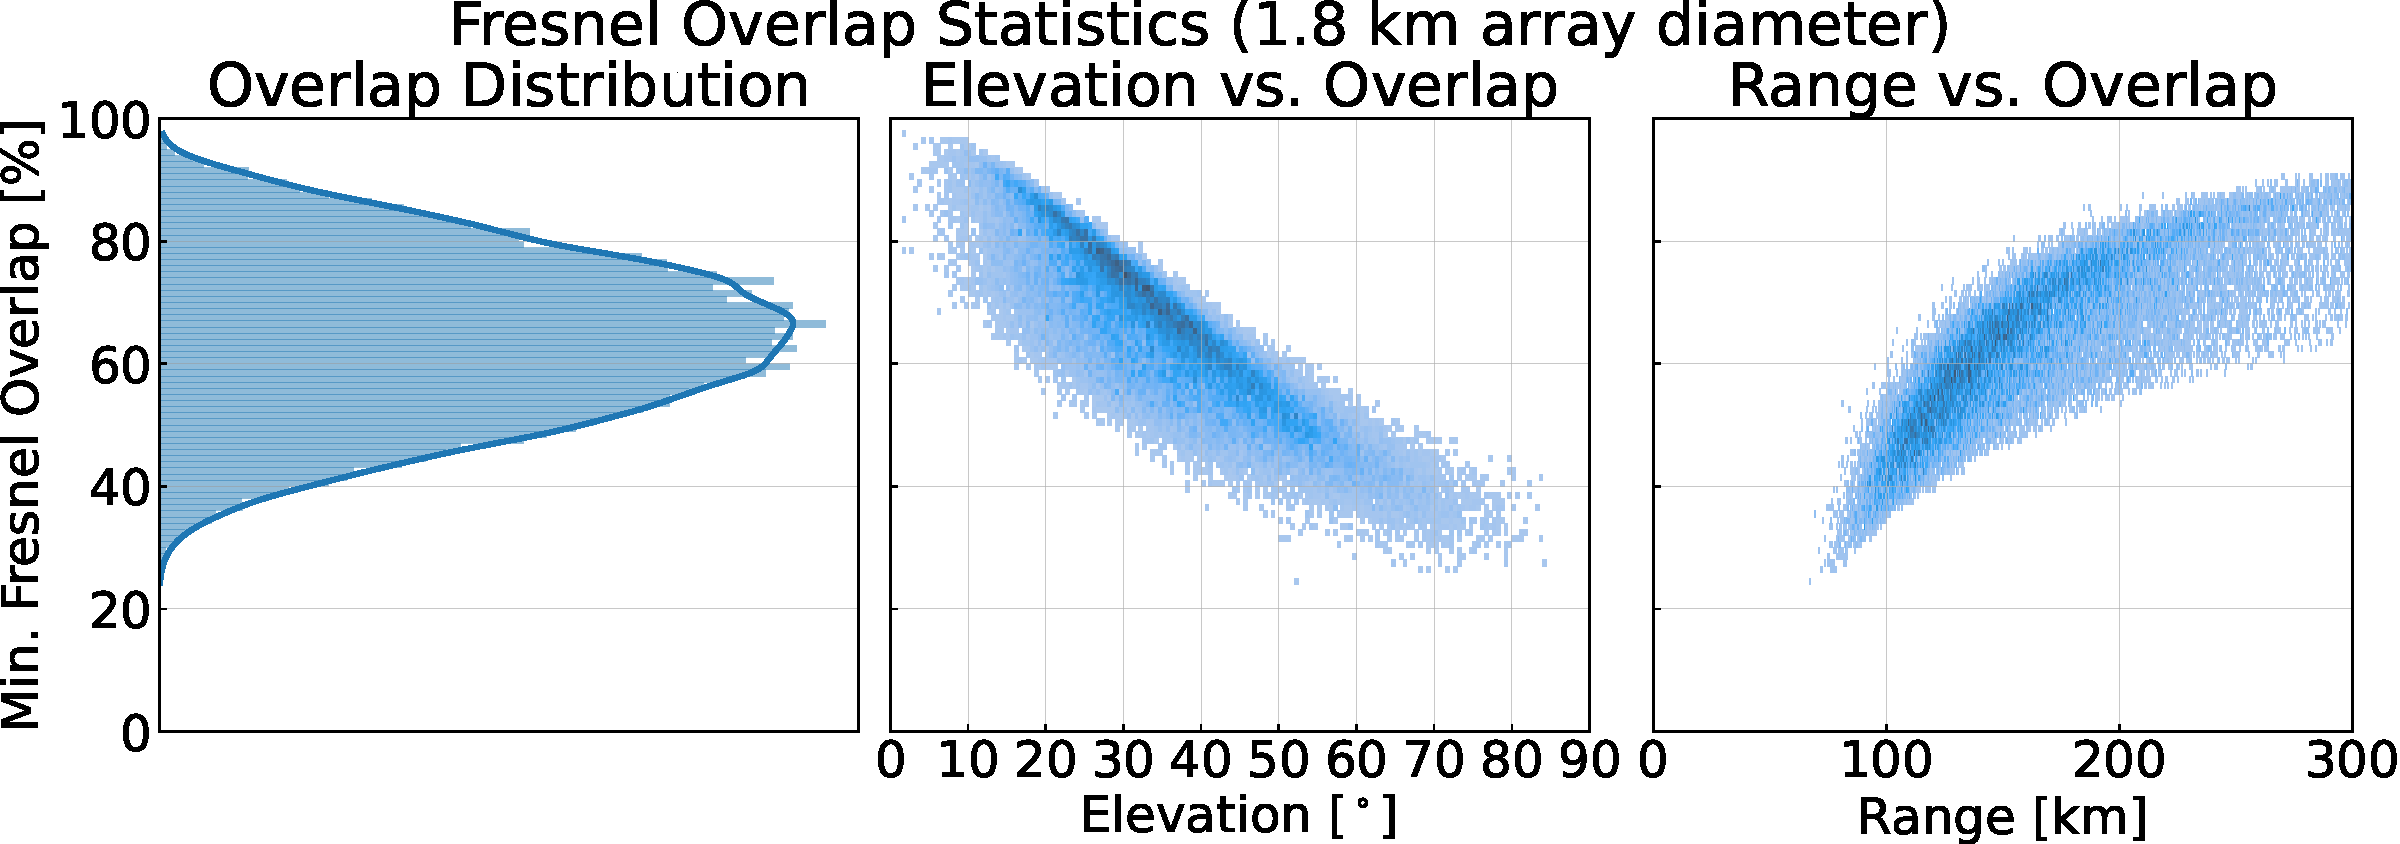
\includegraphics[width=0.8\linewidth]{img/overlap_stats.pdf}
        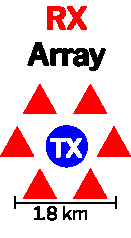
\includegraphics[height=0.35\textheight]{img/rx_array.pdf}
    \end{center}
    \begin{itemize}
        \item[$\blacktriangleright$] \alert{Most meteors seen by all \textcolor{red}{\textbf{RX}}s}: 95\% observations shared by all array members
        \item[$\blacktriangleright$] \alert{Significant Fresnel overlap} 
        \begin{itemize}
            \item 95\% of common observations have >42.9\% overlap
            \item 85\% of common observations have >50\% overlap
        \end{itemize}
    \end{itemize}
\end{frame} 

\begin{frame}[label=errors]
    \frametitle{Results: Errors}
    \begin{center}
        {\colorbox{yellow}{\textbf{Uncertainties match errors}}}
        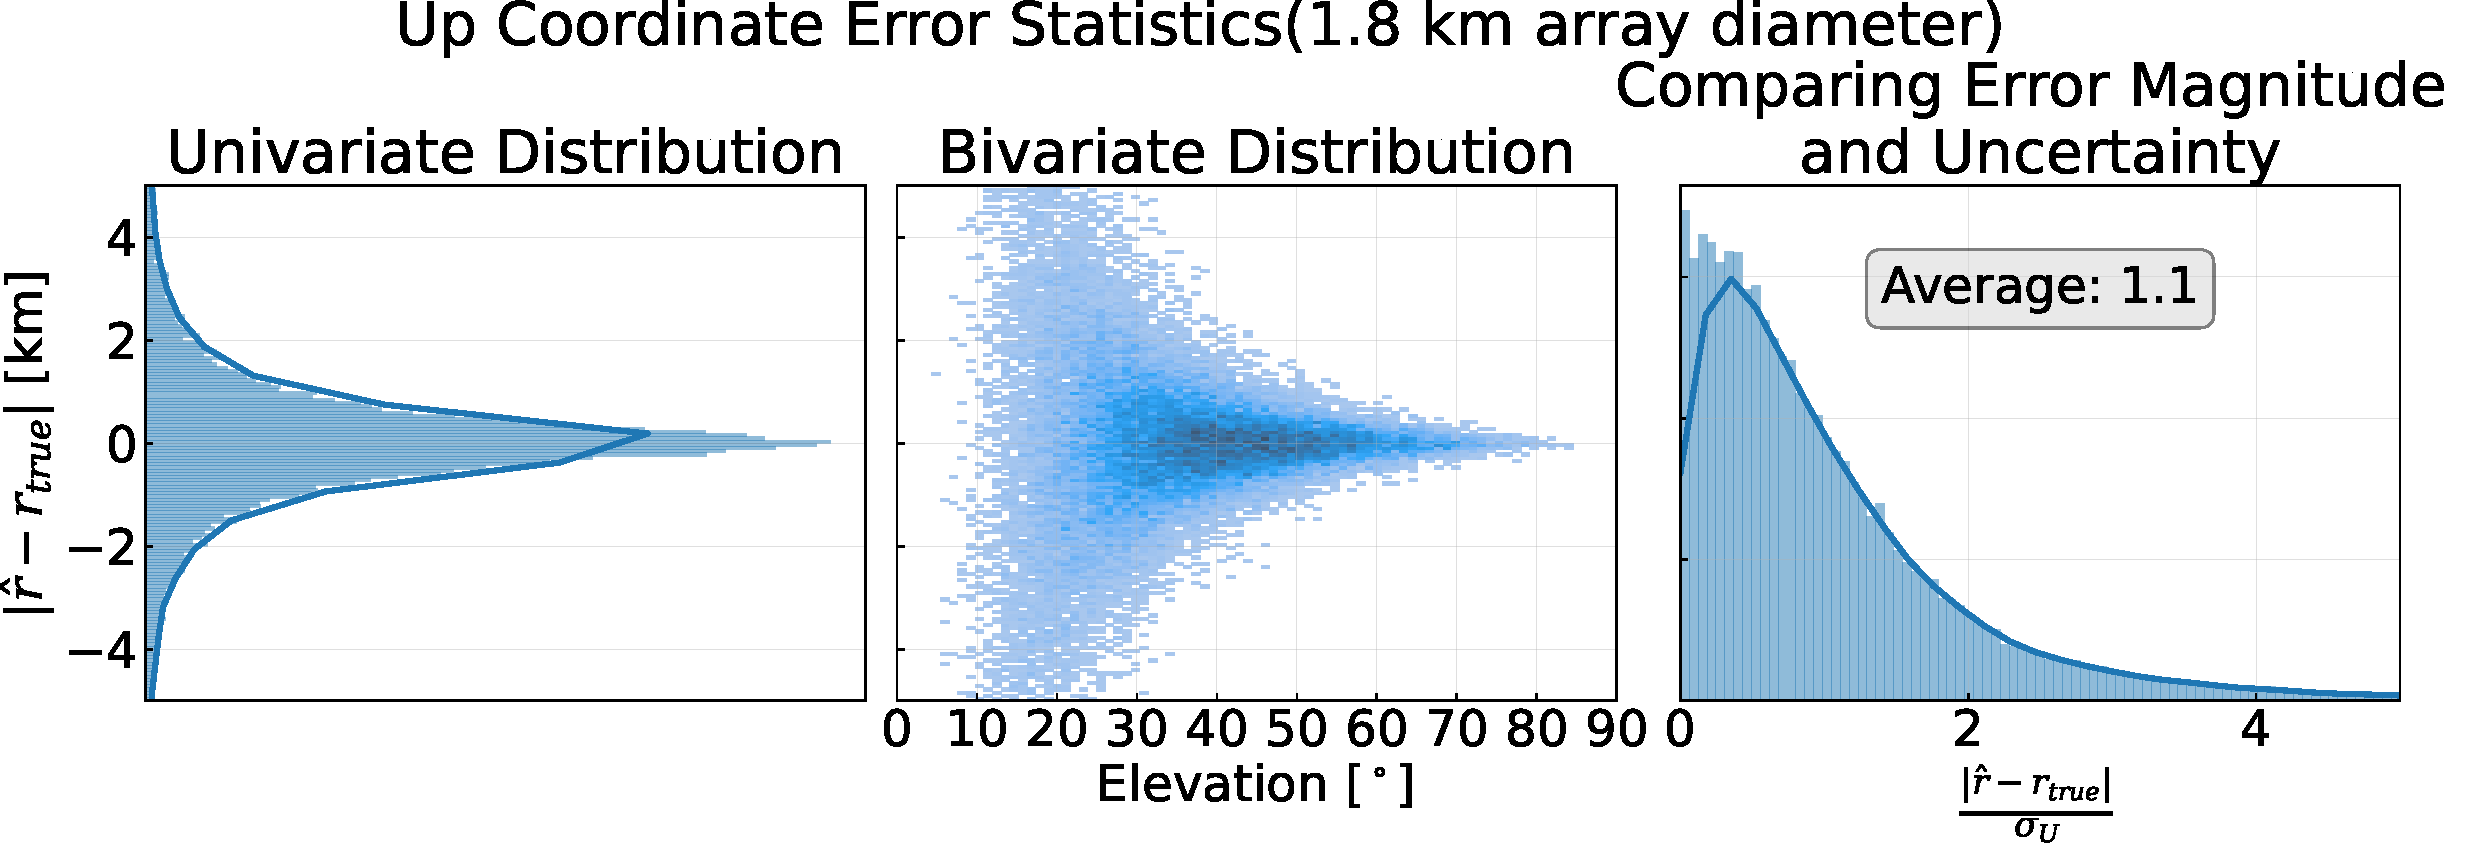
\includegraphics[width=0.8\textwidth]{img/error_stats.pdf}
        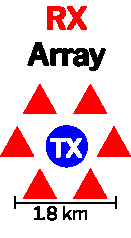
\includegraphics[height=0.35\textheight]{img/rx_array.pdf}
    \end{center}
    \begin{itemize}
        \item Magnitude of positional error is similar to magnitude of reported uncertainties
        \item Smaller errors at high elevation angles
    \end{itemize}
\end{frame}

\section{Future Work and Summary}

\begin{frame}[label=future_work]
    \frametitle{Future Work}
    \begin{columns}
        \begin{column}{0.7\textwidth}
            \begin{itemize}
                \item Verify de-biased correlation function with real data
                \item Examine the effects of error in assumed \textcolor{blue}{\textbf{TX}}/\textcolor{red}{\textbf{RX}} positions 
                \item Carry out experimental campaign to directly compare interferometric and TOF solutions.
            \end{itemize}
            ~ \\ ~ \\ ~ \\ ~
        \end{column}
        \begin{column}{0.4\textwidth}
            \centering
            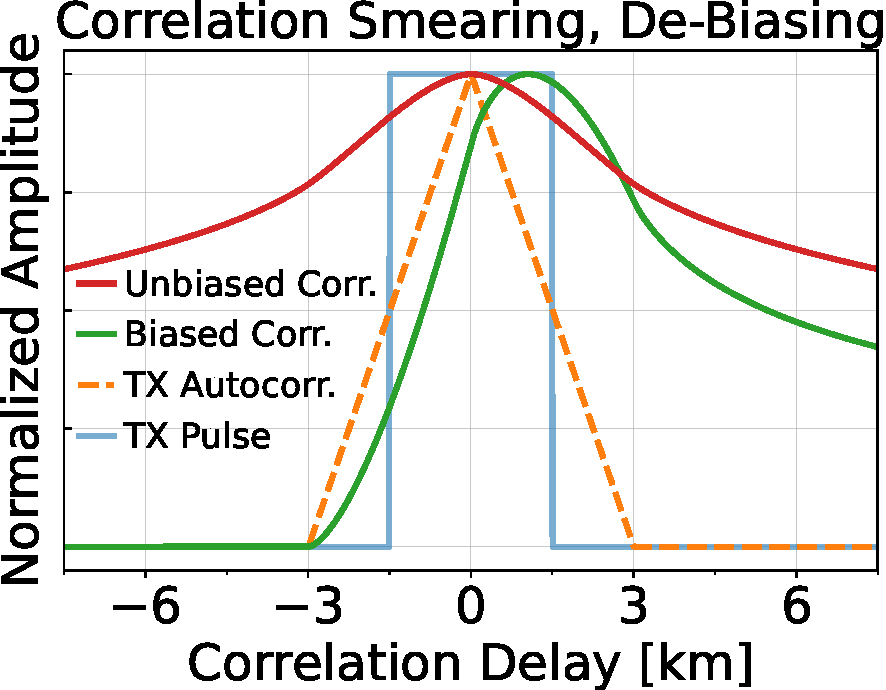
\includegraphics[width=0.65\linewidth]{img/corr_smear_0F1.pdf}
            \\
            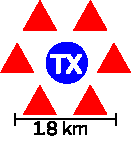
\includegraphics[width=0.2\linewidth]{img/rx_array_unlabeled.pdf}            
             ~ \\ ~ \\ ~ \\ ~ \\ ~ \\ ~ \\ ~ \\ 
        \end{column}
    \end{columns}
    \begin{tikzpicture}[remember picture, overlay]
        \node[anchor=south west] (img) at ([xshift=0.5cm, yshift=0.5cm]current page.south west) {
            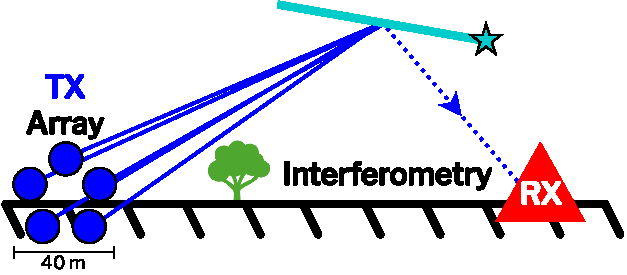
\includegraphics[width=0.45\linewidth]{img/IF_basis_labeled.pdf}%
        };
        \node[anchor=south east] at ([xshift=-0.5cm, yshift=0.5cm]current page.south east) {
            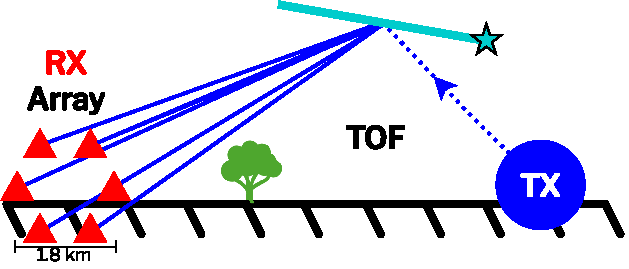
\includegraphics[width=0.45\linewidth]{img/TOF_basis_labeled.pdf}
        };
        \node[anchor=center] at ([yshift=-3cm]current page.center) { 
            vs.
        };
    \end{tikzpicture}
\end{frame}

\begin{frame}[label=gnss_conclusions]
    \frametitle{Summary: Time-of-Flight (TOF) Positioning}
    % \begin{columns}
    %     \begin{column}{1.1\textwidth}
    %         \alert{Specular meteor radar} systems use interferometry to locate reflective meteors and probe the MLT \\ ~ \\
    %     \end{column}
    % \end{columns}
    \begin{columns}
        \begin{column}{0.7\textwidth}
            \alert{Specular meteor radar} systems use interferometry to locate reflective meteors and probe the MLT \\ ~ \\

            \uncover<2->{\alert{Interferometry is challenging} to calibrate, derive uncertainties} \\ ~ \\
            % \begin{itemize}
            %     \item[$\blacktriangleright$] Makes deployment, operation, and analysis difficult 
            % \end{itemize}}

            \uncover<3->{\alert{TOF positioning} can provide precise position estimates %
            \begin{itemize}  %\vspace{-\baselineskip}%
                \item Only uses range measurements
                \item {No calibration} \(\xrightarrow[]{}\) {easier deployments}
                \item {Easily derived uncertainties} \(\xrightarrow[]{}\) {better analysis}
                \item Robust to noise \(\xrightarrow[]{}\) {fewer observations discarded}
            \end{itemize}}

            \uncover<4->{\alert{Few system changes required}: larger \textcolor{red}{\textbf{RX}} arrays} \\ ~ \\ 

            \uncover<5->{Could \alert{replace or supplement} interferometry} \\ ~ \\

            \uncover<6->{An experimental campaign was attempted to directly compare positioning methods}

        \end{column}
        \begin{column}{0.4\textwidth}
            \centering
             \begin{tikzpicture}[anchor=(current bounding box.north)]
                \node[anchor=north, inner sep=0] (img) at (0,0) {
                    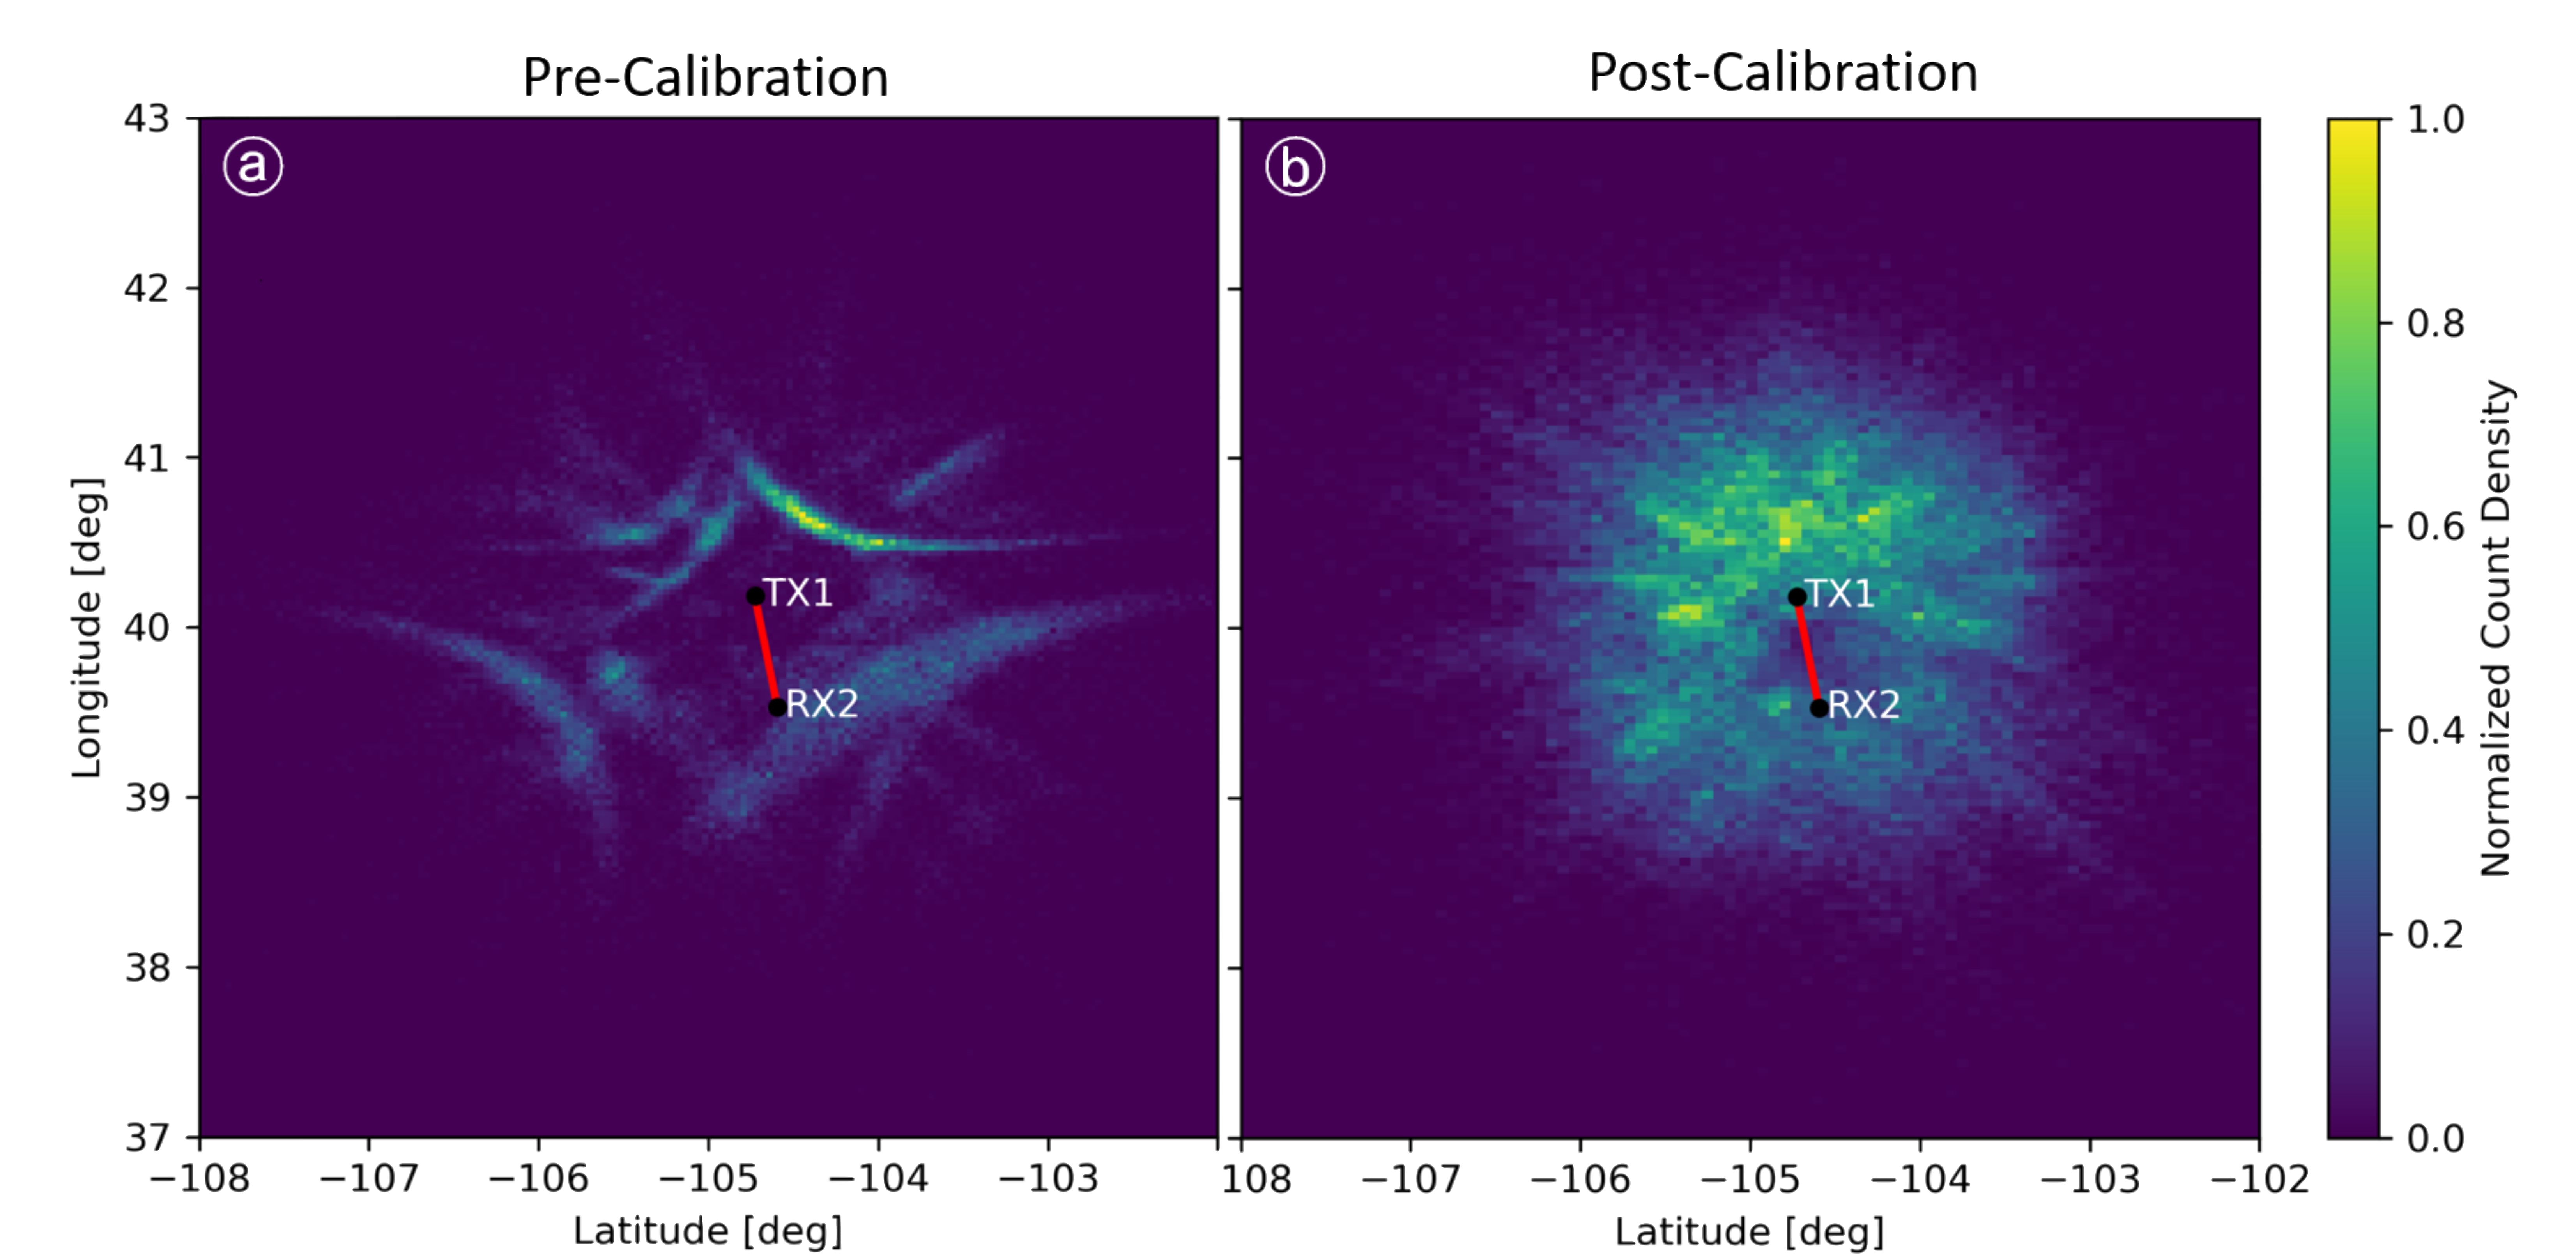
\includegraphics[width=0.85\linewidth]{img/calibration2.png}
                };
                \node[anchor=south, inner sep=2pt] at ([yshift=0.25cm, xshift=0.6cm]img.south) { 
                    {{{\fontsize{3}{3.4}\selectfont\raggedleft \textcolor{white}{\textit{Credit:} \citeauthor{marino_MeteorRadarPhase_2024}, \citeyear{marino_MeteorRadarPhase_2024} \cite{marino_MeteorRadarPhase_2024}}}}}
                };
            \end{tikzpicture}
            % 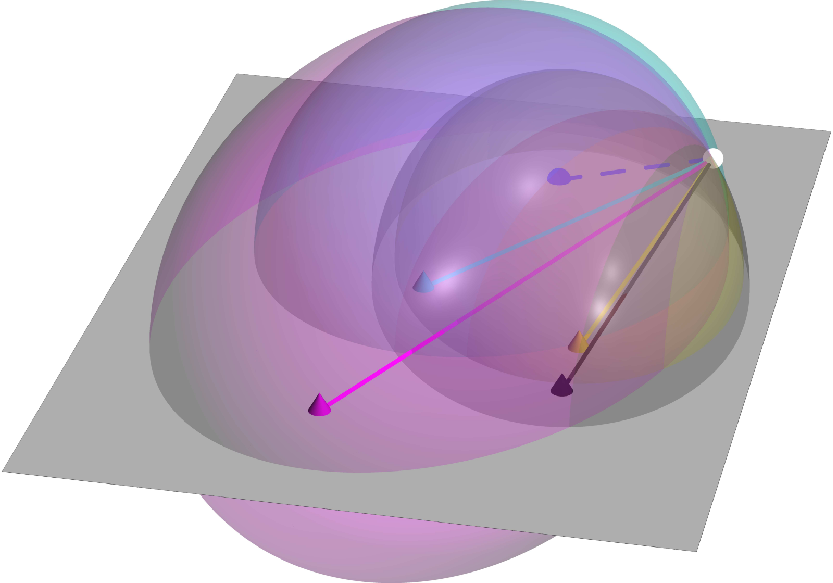
\includegraphics[width=0.65\linewidth]{img/4ellipsoids_compressed.pdf}
            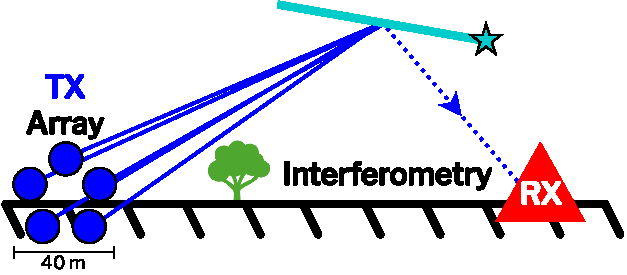
\includegraphics[width=\linewidth]{img/IF_basis_labeled.pdf}
            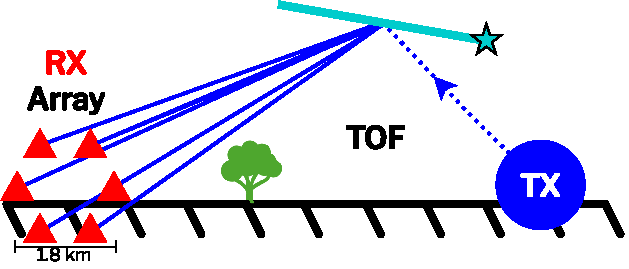
\includegraphics[width=\linewidth]{img/TOF_basis_labeled.pdf}
        \end{column}
    \end{columns}
\end{frame}

% Q&A
\begin{frame}[standout]
    \Huge\textsc{Thank You}

    \vfill
    
    \LARGE\textsc{Questions? Job offers?}
    \textsc{Email: jamo8071@colorado.edu}
\end{frame}

\begin{frame}[allowframebreaks]
    \frametitle{References}
    \printbibliography[heading=none]
\end{frame}


% \appendix
% \begin{frame}[label=gnss_ls_bk]
    \frametitle{GNSS: Developing a Least Squares Estimator}
    With 4+ bistatic range measurements, the meteor trail's reflection point can be estimated: 
    \begin{columns}
        \begin{column}{0.5\textwidth}
            {\setlength{\leftmargini}{1em} \begin{enumerate}
                \item Develop a \alert{ measurement model}, relating:  
                \begin{columns}
                    \begin{column}{0.5\linewidth }
                        {\setlength{\leftmargini}{3em} \begin{itemize} \scriptsize
                            \item[\(\blacktriangleright\)] \(\rho\): bistatic range
                            \item[\(\blacktriangleright\)] \(\mathbf{r}^{T}\): \textcolor{blue}{\textbf{TX}} location
                        \end{itemize}}
                    \end{column}
                    \begin{column}{0.5\linewidth}
                        \begin{itemize} \scriptsize
                            \item[\(\blacktriangleright\)] \(\mathbf{r}^R\): \textcolor{red}{\textbf{RX}} location
                            \item[\(\blacktriangleright\)] \(\mathbf{r}^s\): reflection point 
                        \end{itemize}
                    \end{column}
                \end{columns}                
            \end{enumerate}}
        \end{column}
        \begin{column}{0.5\textwidth}
            \scriptsize \begin{equation*} 
                \rho\left( \mathbf{r}^{s} \right) = \sqrt{\left( \mathbf{r}^{R}-\mathbf{r}^{s} \right)^{2}} + \sqrt{\left( \mathbf{r}^{T}-\mathbf{r}^{s} \right)^{2}} + \varepsilon
            \end{equation*}
        \end{column}
    \end{columns}
    %
    \begin{columns}
        \begin{column}{0.5\textwidth}
            {\setlength{\leftmargini}{1em} \begin{enumerate}   \setcounter{enumi}{1}
                \item \alert{Linearize the model} about some initial guess \(\mathbf{r}_0^s\)
            \end{enumerate}}
        \end{column}
        \begin{column}{0.5\textwidth}
            \scriptsize \begin{equation*}
                \rho \left( \mathbf{r}^{s} \right) \approx  \rho\left( \mathbf{r}^{s}_{0} \right) + \left. \frac{\partial \rho}{\partial \mathbf{r}^{s} } \right|_{\mathbf{r}^{s} = \mathbf{r}^{s}_0} \left( \mathbf{r}^{s} - \mathbf{r}^{s}_{0} \right)^{\top}
            \end{equation*}
        \end{column}
    \end{columns}
    %
    \begin{columns}
        \begin{column}{0.5\textwidth}
             {\setlength{\leftmargini}{1em} \begin{enumerate}   \setcounter{enumi}{2}
                \item \alert{Solve for the deviation} from the initial guess, \(\delta \mathbf{r} = \mathbf{r}^{s} - \mathbf{r}^{s}_{0}\)
            \end{enumerate}}
        \end{column}
        \begin{column}{0.5\textwidth}
            \scriptsize \begin{equation*}
                 \delta\rho =  \rho\left( \mathbf{r}^{s} \right)  -  \rho\left( \mathbf{r}^{s}_{0} \right) = \left. \frac{\partial \rho}{\partial \mathbf{r}^{s} } \right|_{\mathbf{r}^{s} = \mathbf{r}^{s}_0} \delta \mathbf{r}^{\top} + \varepsilon
            \end{equation*}
        \end{column}
    \end{columns}
    %
    \begin{columns}
        \begin{column}{0.5\textwidth}
            {\setlength{\leftmargini}{1em} \begin{enumerate}   \setcounter{enumi}{3}
                \item Put into \alert{least squares formulation} to find best position solution
            \end{enumerate}}
        \end{column}
        \begin{column}{0.5\textwidth}
            \scriptsize \begin{equation*}
                \delta\boldsymbol{\rho} = \mathbf{G}  \delta \mathbf{r}^{\top} + \boldsymbol{\varepsilon} \xrightarrow[]{}  \delta \hat{\mathbf{r}} = \left( \mathbf{G}^{\top} \mathbf{G} \right)^{-1} \mathbf{G}^{\top} \delta \boldsymbol{\rho}
            \end{equation*}
        \end{column}
    \end{columns}
    %
    \begin{columns}
        \begin{column}{0.5\textwidth}
            {\setlength{\leftmargini}{1em} \begin{enumerate}   \setcounter{enumi}{4}
                \item \alert{Update the initial guess}: set \(\mathbf{r}_0^s = \hat{\mathbf{r}}\)
            \end{enumerate}}
        \end{column}
        \begin{column}{0.5\textwidth}
            \scriptsize \begin{equation*}
                \hat{\mathbf{r}} = \mathbf{r}_0^s + \delta \hat{\mathbf{r}}
            \end{equation*}
        \end{column}
    \end{columns}
    %
    \begin{columns}
        \begin{column}{0.5\textwidth}
            {\setlength{\leftmargini}{1em} \begin{enumerate} \setcounter{enumi}{5}
                \item \alert{Repeat} until convergence
            \end{enumerate}}
        \end{column}
        \begin{column}{0.5\textwidth}
            
        \end{column}
    \end{columns}
\end{frame}

\begin{frame}[t, label=missed_weak]
    \frametitle{What Meteors are Missed?}
    \centering
    A: \alert{Weak reflection} towards \textcolor{red}{\textbf{RX}} \uncover<2->{\(\xrightarrow[]{}\) \alert{Increase \textcolor{blue}{\textbf{TX}} power}}

    \begin{tikzpicture}[remember picture, overlay]
        \node<1>[anchor=south east] (img) at ([xshift=-0.1cm, yshift=0.55cm]current page.south east) {
            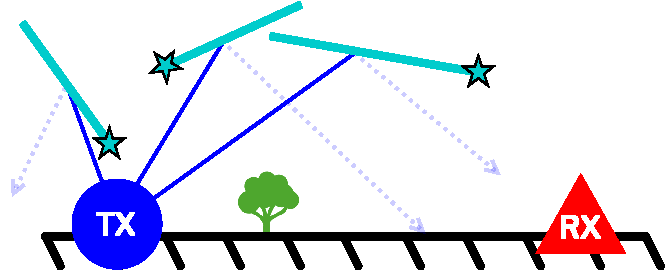
\includegraphics[height=6cm]{img/improve_link.pdf}%
        };
        \node<2->[anchor=south east] at ([xshift=-0.1cm, yshift=0.55cm]current page.south east) {
            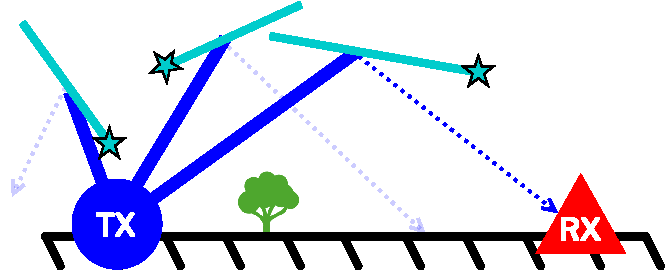
\includegraphics[height=6cm]{img/increase_power.pdf}%
        };
        \node[circle, draw=yellow, fill=yellow!30, thick, minimum size=4mm] at ([xshift=1.85cm, yshift=-1.5cm]img.north west) {C};
        \node[circle, draw=yellow, fill=yellow!30, thick, minimum size=4mm] at ([xshift=-2.25cm, yshift=-0.35cm]img.north) {B};
        \node[circle, draw=yellow, fill=yellow!30, thick, minimum size=4mm] at ([xshift=0.4cm, yshift=-0.6cm]img.north) {A};
    \end{tikzpicture}
\end{frame}

\begin{frame}[t, label=missed_away]
    \frametitle{What Meteors are Missed?}
    \centering
    B: Reflects power within network, \alert{away from \textcolor{red}{\textbf{RX}}} \uncover<2->{\(\xrightarrow[]{}\) \alert{Increase network density}}

    \begin{tikzpicture}[remember picture, overlay]
        \node<1>[anchor=south east] (img) at ([xshift=-0.1cm, yshift=0.55cm]current page.south east) {
            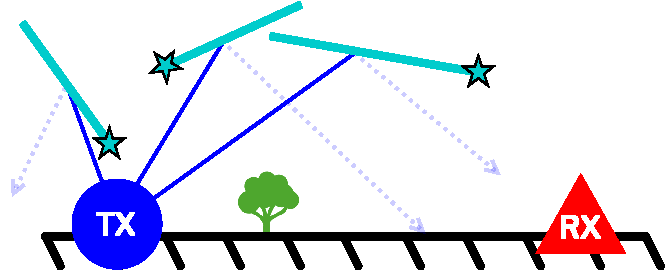
\includegraphics[height=6cm]{img/improve_link.pdf}%
        };
        \node<2->[anchor=south east] at ([xshift=-0.1cm, yshift=0.55cm]current page.south east) {
            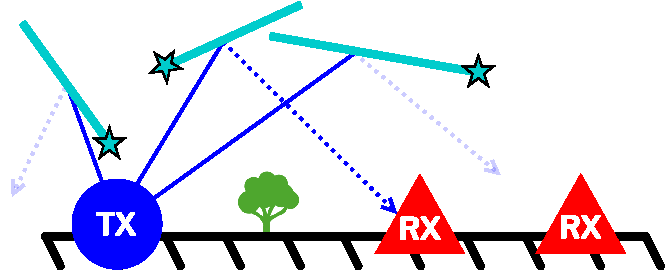
\includegraphics[height=6cm]{img/increase_density.pdf}%
        };
        \node[circle, draw=yellow, fill=yellow!30, thick, minimum size=4mm] at ([xshift=1.85cm, yshift=-1.5cm]img.north west) {C};
        \node[circle, draw=yellow, fill=yellow!30, thick, minimum size=4mm] at ([xshift=-2.25cm, yshift=-0.35cm]img.north) {B};
        \node[circle, draw=yellow, fill=yellow!30, thick, minimum size=4mm] at ([xshift=0.4cm, yshift=-0.6cm]img.north) {A};
    \end{tikzpicture}
\end{frame}

\begin{frame}[t, label=missed_outside]
    \frametitle{What Meteors are Missed?}
    \centering
    C: Reflects power \alert{outside network} \uncover<2->{\(\xrightarrow[]{}\) \alert{Increase network coverage}}

    \begin{tikzpicture}[remember picture, overlay]
        \node<1>[anchor=south east] (img) at ([xshift=-0.1cm, yshift=0.55cm]current page.south east) {
            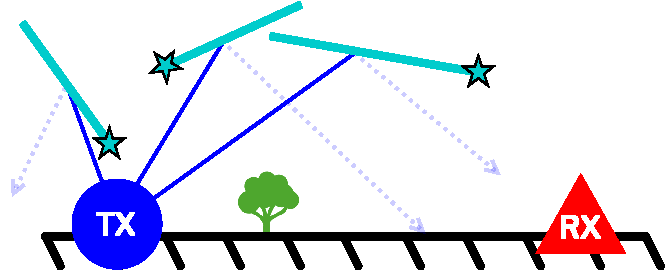
\includegraphics[height=6cm]{img/improve_link.pdf}%
        };
        \node<2->[anchor=south east] at ([xshift=-0.1cm, yshift=0.55cm]current page.south east) {
            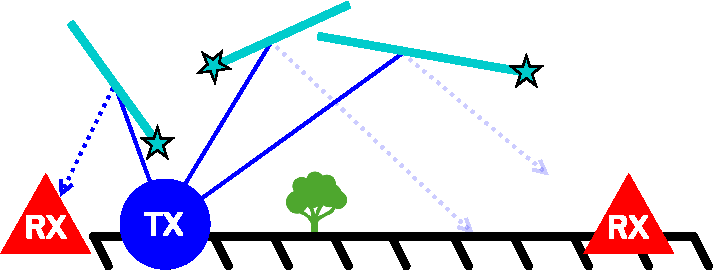
\includegraphics[height=6cm]{img/increase_coverage.pdf}%
        };
        \node[circle, draw=yellow, fill=yellow!30, thick, minimum size=4mm] at ([xshift=1.85cm, yshift=-1.5cm]img.north west) {C};
        \node[circle, draw=yellow, fill=yellow!30, thick, minimum size=4mm] at ([xshift=-2.25cm, yshift=-0.35cm]img.north) {B};
        \node[circle, draw=yellow, fill=yellow!30, thick, minimum size=4mm] at ([xshift=0.4cm, yshift=-0.6cm]img.north) {A};
    \end{tikzpicture}
\end{frame} 

\end{document}